\chapter{参数化研究}\label{chap:parametric}

\section{参数化研究设计框架}

\subsection{设计变量与工况矩阵}

依照单因素变化原则，本课题共设计三组别20个喷嘴工况，分别调整喷嘴收缩角$\theta$、喷嘴竖向长度$L$、整形板倾斜角$\alpha$以及整形板延伸长度$TL$四个控制变量，分别设计4-5组不同工况，研究喷嘴参数（A组）、整形板参数（B组）对混凝土喷嘴挤出机制的影响，并同时设计对照优化组（C组），探索四控制变量下的最优解。

定义工况的几何参数矩阵如\cref{tab:4.1}所示。

\begin{table}[!htb]
  \centering
  \caption{工况完整参数矩阵与 $P_{sub,AWA}$ 结果}\label{tab:4.1}
  \renewcommand{\arraystretch}{1.2}
  \footnotesize
  \begin{tabular}{lccccccp{3cm}}
    \toprule
    \textbf{工况} & $TL$ & $\theta$ & $L$ & $\alpha$ & $H$ (mm) & $P_{sub,AWA}$ (Pa) & \textbf{组别说明} \\
    \midrule
    Baseline & 50 & 30° & 20 & 10° & 13.32 & 8310  & 基准工况 \\
    A1-1     & 50 & 15° & 20 & 10° & 13.32 & 8286  & 研究线A1：$\theta$变化 \\
    A1-2     & 50 & 0°  & 20 & 10° & 13.32 & 8357  &  \\
    A1-3     & 50 & 45° & 20 & 10° & 13.32 & 9130  &  \\
    A1-4     & 50 & 60° & 20 & 10° & 13.32 & 9926  &  \\
    A2-1     & 50 & 30° & 10 & 10° & 13.32 & 8323  & 研究线A2：$L$变化 \\
    A2-2     & 50 & 30° & 30 & 10° & 13.32 & 8905  &  \\
    A2-3     & 50 & 30° & 40 & 10° & 13.32 & 9382  &  \\
    B1-1     & 50 & 30° & 20 & 0°  & 22.00 & 5733  & 研究线B1：$\alpha$变化 \\
    B1-2     & 50 & 30° & 20 & 5°  & 17.64 & 6896  &  \\
    B1-3     & 50 & 30° & 20 & 15° & 9.06  & 12081 &  \\
    B1-4     & 50 & 30° & 20 & 20° & 4.90  & 22184 &  \\
    B2-1     & 30 & 30° & 20 & 10° & 16.79 & 5944  & 研究线B2：$TL$变化 \\
    B2-2     & 40 & 30° & 20 & 10° & 15.05 & 7177  &  \\
    B2-3     & 60 & 30° & 20 & 10° & 11.58 & 10353 &  \\
    B2-4     & 70 & 30° & 20 & 10° & 9.85  & 12833 &  \\
    C1-1     & 50 & 60° & 20 & 10° & 13.32 & 9926  & C组：A组最优 \\
    C1-2     & 55 & 30° & 20 & 15° & 7.77  & 14525 & C组：Trowel优化 \\
    C1-3     & 60 & 60° & 20 & 15° & 6.47  & 21677 & C组：性能最优 \\
    C2       & 0  & 30° & 20 & 10° & 22.00 & 3436  & C组：无顶板对照组 \\
    C3       & 60 & 60° & 20 & 15° & 6.47  & 21702 & C组：含Fillet几何优化 \\
    \bottomrule
  \end{tabular}
\end{table}

\subsection{评价指标定义}

喷嘴的性能评价是一个复杂的多目标体系，其几何特征会直接影响能效传递、层间粘结性能、材料损伤风险、泵送经济性、压力均匀性等等方面，而在实际工程实践当中，往往需要对这些指标进行综合评判，找到一个性能最优的解决方案。本课题定义了五项评价指标，从多个角度对喷嘴工况的表现进行量化与评价。

（1）基底面积加权平均压力$P_{sub,AWA}$：基底面积加权平均压力$P_{sub,AWA}$是本课题最核心的评价指标之一，定义为打印基底面上各网格单元静压力以面积为权重的加权平均值。这项指标是整形板对浆体施加的平均接触压力的反映，可以间接反映层间粘结强度。较高的接触压力有助于压实层间界面，促进水泥浆料的界面融合，提升层间抗剪和抗拉强度。

（2）喷嘴出口截面壁面剪切应力$WSS_{nozzle}$：喷嘴出口截面壁面剪切应力$WSS_{nozzle}$是喷嘴出口处壁面剪切应力的面积加权平均值。这个指标反映了喷嘴内壁在出口区域所承受的切向摩擦载荷，与喷嘴磨损速率正相关；于此同时，过高的剪切应力可能导致打印混凝土浆体的结构网络被过度破坏，影响挤出后的形状保持能力与早龄期强度发展。

（3）压力传递效率$\eta_p$：压力传递效率$\eta_p$是基底面面积加权平均压力与入口面积加权平均压力之比，公式表达为：
\begin{equation}\label{eq:eta-p}
  \eta_p = \frac{P_{sub,AWA}}{P_{inlet,AWA}}.
\end{equation}
该指标反映了泵送系统施加的驱动压力中，最终转化为基底有效接触压力的比例，是衡量打印系统压力利用经济性的无量纲指标。$\eta_p$越大，说明系统在相同泵送能耗下能够产生更高的层间接触压力，系统整体效率越高。

（4）压力非均匀性指数$UI$（Uniformity Index）：压力非均匀性指数$UI$是基底面压力最大值与最小值之差相对于面积加权平均压力的比值，公式表达为：
\begin{equation}\label{eq:UI}
  UI = \frac{P_{sub,Max} - P_{sub,Min}}{P_{sub,AWA}}.
\end{equation}
压力非均匀性指数反映了基底面接触压力的空间分布均匀程度。$UI$越小，整形板对基底面的压力分布越均匀，有利于层间粘结质量的空间一致性；$UI$过大，意味着局部压力集中，可能导致层间粘结强度的空间不均匀。

（5）入口面积加权平均压力$P_{inlet}$：$P_{inlet}$作为泵送能耗的代理指标，反映了打印系统维持稳定挤出所需的泵送驱动压力。$P_{inlet}$越小，对泵送设备的压力要求越低，打印系统的能耗与设备成本越低。

\section{喷嘴收缩角$\theta$的影响（A1组工况）}

为研究喷嘴收缩角度对喷嘴挤出性能的影响，本课题共选取5组工况进行了参数化研究。\cref{tab:4.2}总结了5组工况重点研究指标的结果。

\begin{table}[!htb]
  \centering
  \caption{A1组（$\theta$变化）各工况评价指标汇总表}\label{tab:4.2}
  \renewcommand{\arraystretch}{1.3}
  \begin{tabular}{lccccccl}
    \toprule
    \textbf{工况} & $\theta$ & $P_{sub}$(Pa) & $WSS_{nozzle}$ & $\eta_p$ & $UI$ & $P_{inlet}$ & \textbf{综合} \\
    \midrule
    A1-1     & 15° & 8286  & 96.9 & 0.401 & 1.73 & 20685 & \\
    A1-2     & 0°  & 8357  & 89.3 & 0.370 & 1.75 & 22584 & \\
    Baseline & 30° & 8310  & 84.9 & 0.421 & 1.78 & 19750 & \\
    A1-3     & 45° & 9130  & 64.4 & 0.426 & 1.76 & 21451 & \\
    A1-4     & 60° & 9926  & 35.0 & 0.447 & 1.84 & 22190 & 最优 \\
    \bottomrule
  \end{tabular}
\end{table}

\subsection{$\theta$对基底压力的影响}

五种收缩角工况下的压力云图如\cref{fig:4.1}所示，$P_{sub,AWA}$随收缩角$\theta$变化的折线图如\cref{fig:4.2}所示。

\begin{figure}[!htb]
  \centering
  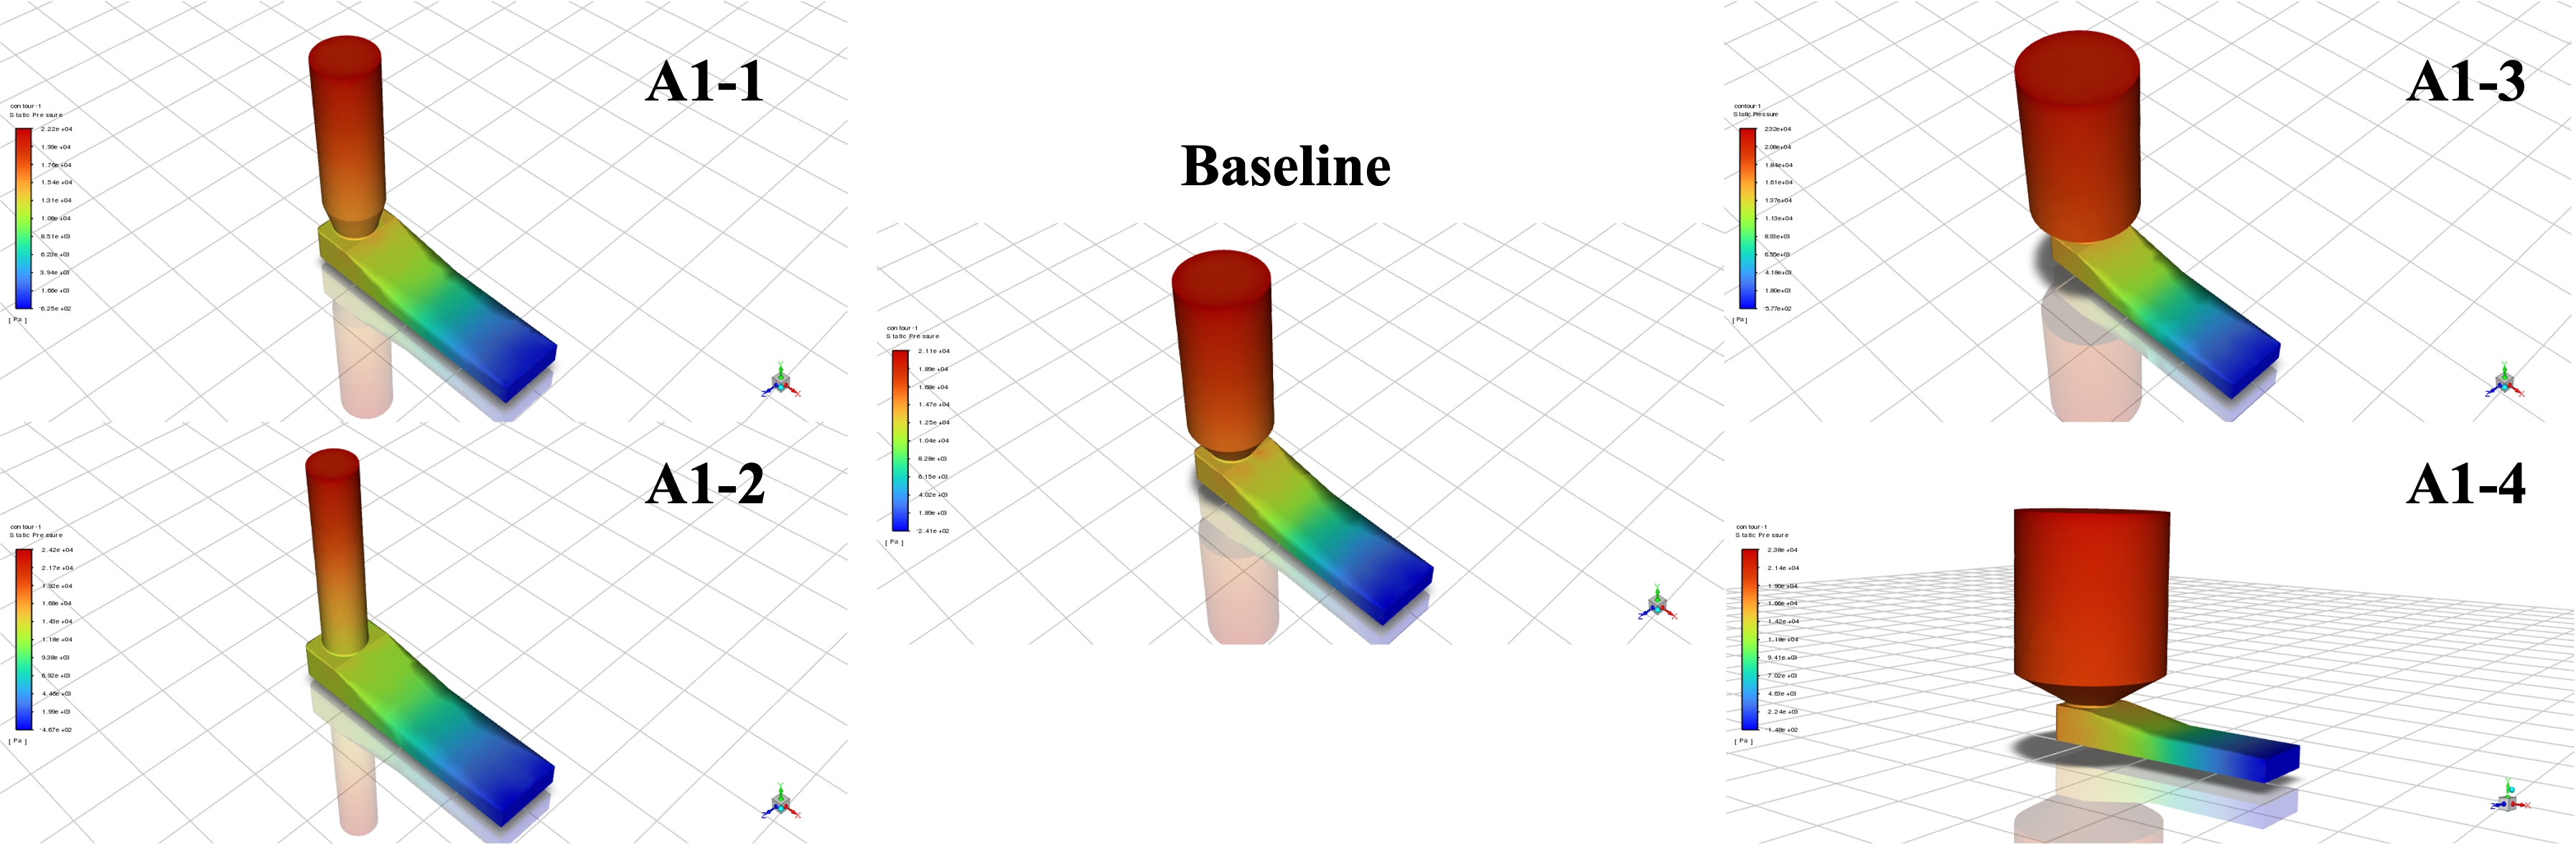
\includegraphics[width=0.9\textwidth]{figures/4.1.png}
  \caption{不同$\theta$下纵截面压力云图对比图}
  \label{fig:4.1}
\end{figure}

\begin{figure}[!htb]
  \centering
  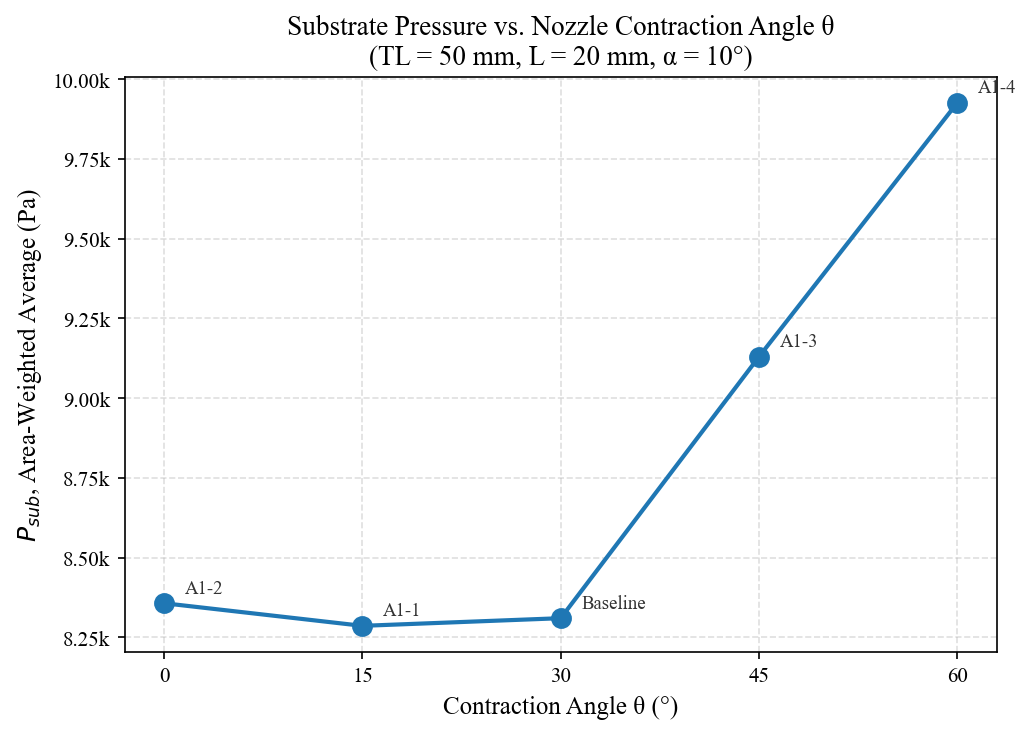
\includegraphics[width=0.75\textwidth]{figures/4.2.png}
  \caption{$P_{sub,AWA}$--$\theta$变化折线图}
  \label{fig:4.2}
\end{figure}

由图可见，随着收缩角$\theta$从0°增大至60°，$P_{sub,AWA}$大致呈平坦-递增趋势，从8286-8357~Pa（$\theta = 0°, 15°, 30°$）增大至9926~Pa（$\theta = 60°$，A1-4工况），增幅为+19\%。收缩角度影响基底压力的机理可能有：

（1）收缩角越大，流道截面积沿轴向的收缩越剧烈，浆体在收缩段内受到更强的径向压缩作用，出口截面处的流速分布更为集中，出口动压更高。根据伯努利方程的定性分析，更高的出口动压在被前挡板阻挡后，能够转化为更大的静压，从而提升基底接触压力。

（2）收缩段几何形状影响喷嘴内部的整体压力分布。由\cref{tab:4.2}中各工况的喷嘴出口压力数据可见，$\theta = 60°$时$P_{nozzle} = 17274$~Pa，显著高于$\theta = 30°$基准工况的13536~Pa，说明更大的收缩角在喷嘴收缩段本身积累了更高的压力，这一压力通过流体传递至下游整形板区域，最终作用于基底面。

另外，A1-2工况的喷嘴收缩角度为0，此时喷嘴组合体是一个退化的工况，喷嘴与直管段形成了一个高度为120~mm的圆柱体。在这个工况之下，喷嘴不再存在有任何收缩效应，喷嘴出口压力为$P_{nozzle} = 13645$~Pa，$P_{sub,AWA}$也不再遵循单调递增趋势，而是稍微高于收缩角为15°与30°的工况。

由以上分析可以看出：缺乏收缩段的加速作用，流体动能未得到充分提升，出口动压和基底接触压力就不会很高。这充分说明了喷嘴收缩段几何形状对喷嘴性能的重要性。

\subsection{$\theta$对喷嘴剪切应力的影响}

不同$\theta$工况下喷嘴出口处壁面剪切应力柱状图对比与整体壁面剪切应力云图对比分别由\cref{fig:4.3}、\cref{fig:4.4}所示。

\begin{figure}[!htb]
  \centering
  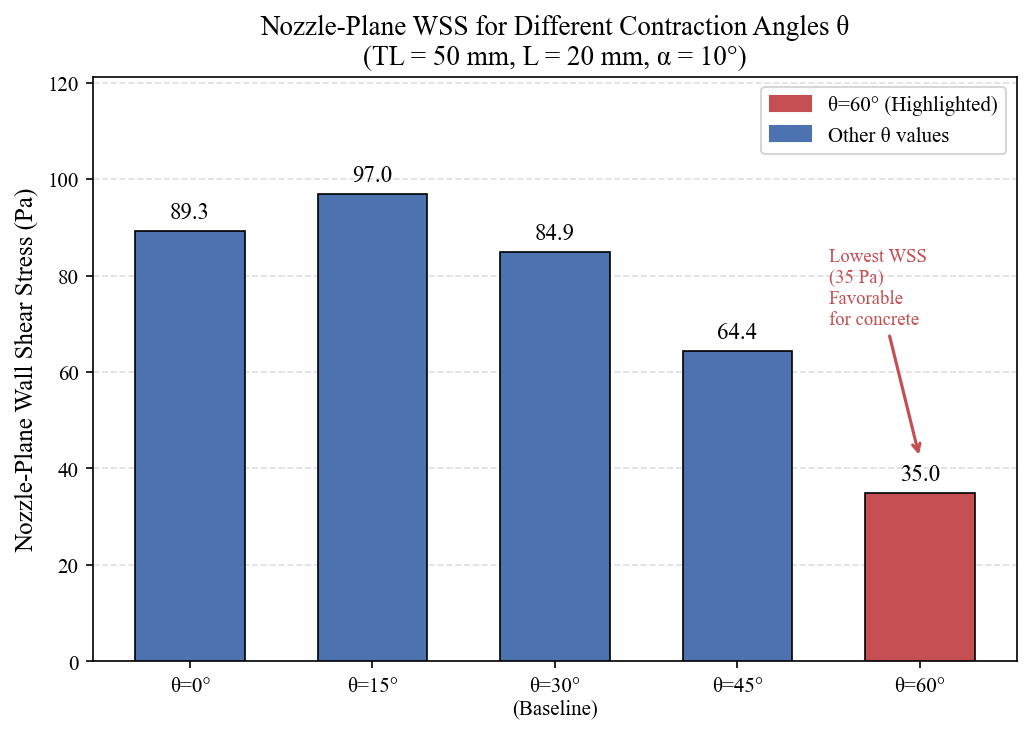
\includegraphics[width=0.75\textwidth]{figures/4.3.png}
  \caption{不同$\theta$工况下喷嘴出口处壁面剪切应力柱状对比图}
  \label{fig:4.3}
\end{figure}

\begin{figure}[!htb]
  \centering
  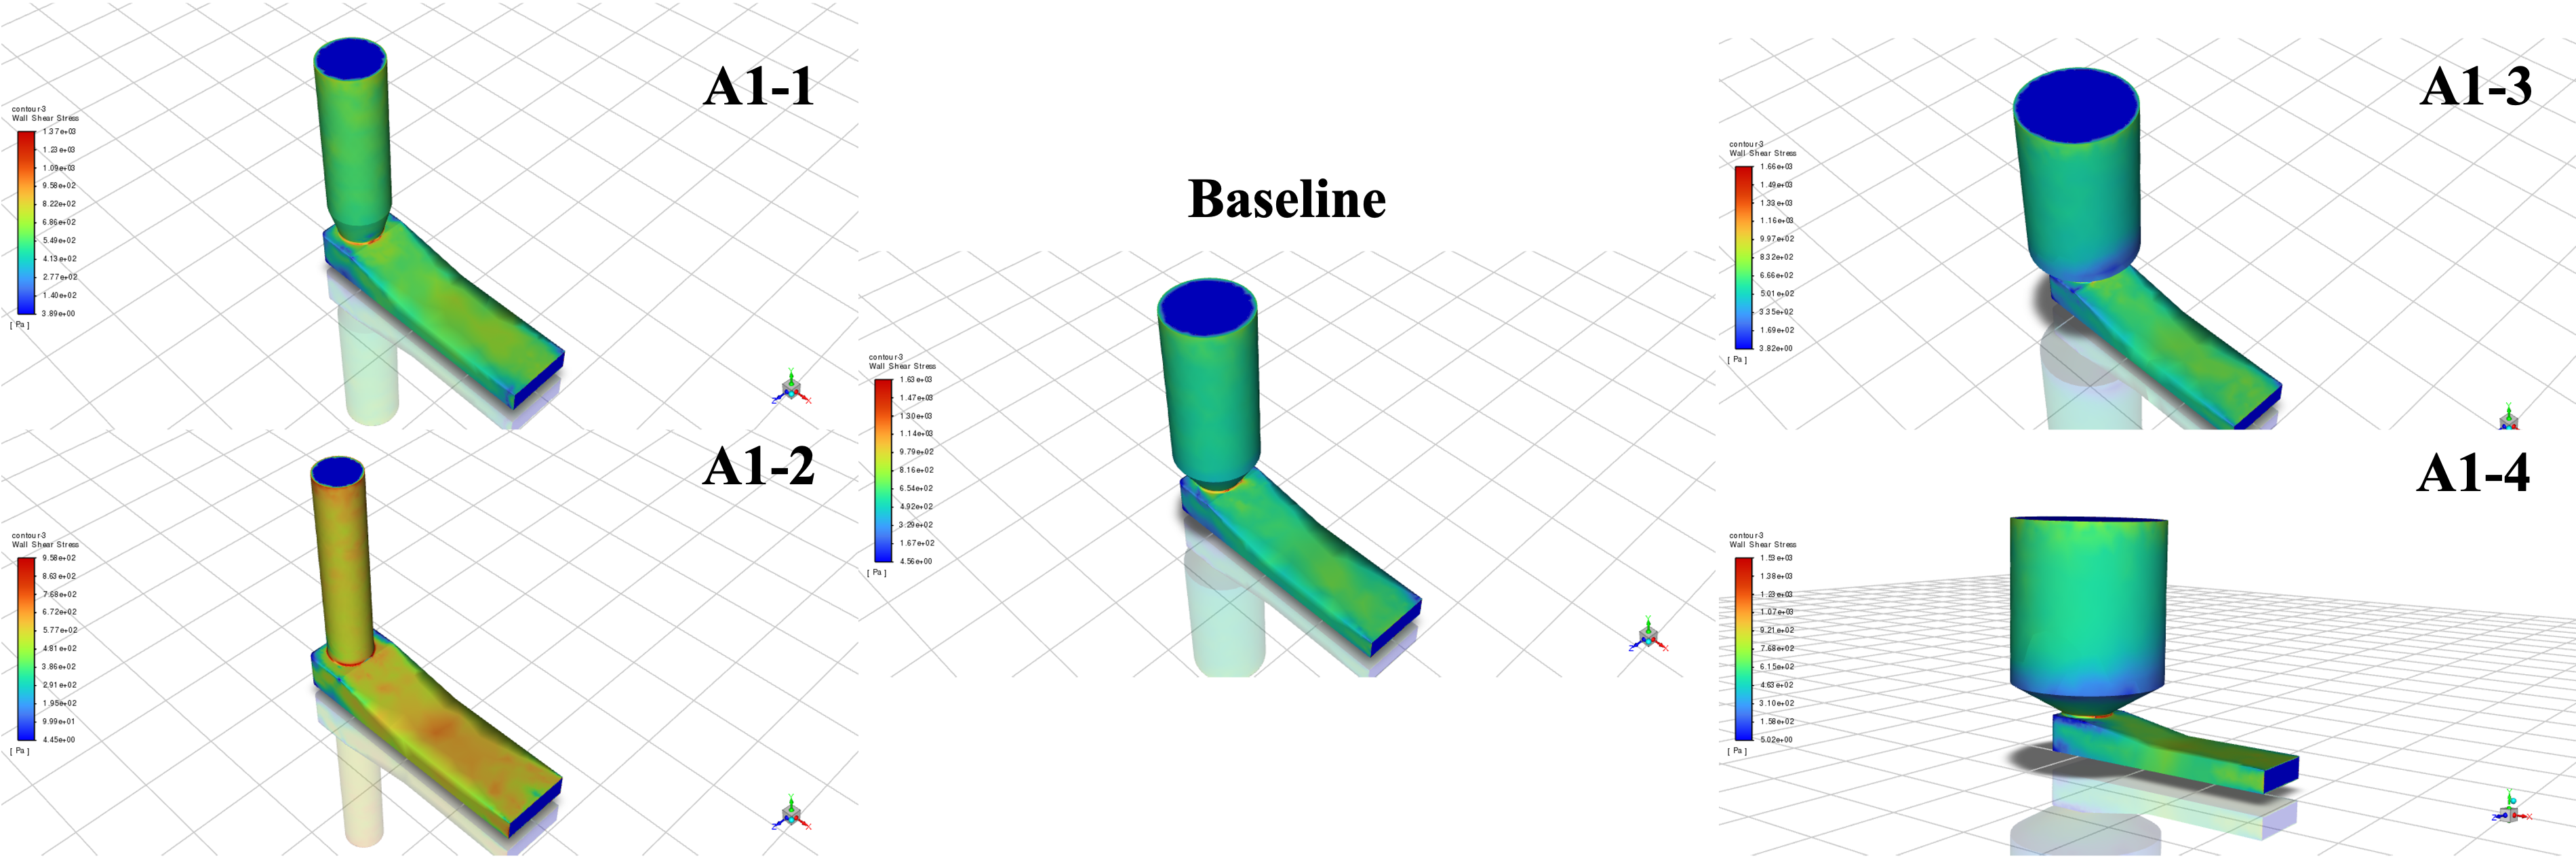
\includegraphics[width=0.9\textwidth]{figures/4.4.png}
  \caption{不同$\theta$下整体壁面剪切应力云图对比图}
  \label{fig:4.4}
\end{figure}

随$\theta$从0°增大至60°，$WSS_{nozzle}$呈现先升再减的趋势，从0°时的89.3~Pa短暂增加到15°时的97.0~Pa，随后单调降低至35.0~Pa，降幅达61\%。这一趋势与$P_{sub,AWA}$随$\theta$增大而先短暂降低后显著升高的规律方向相同，表明$\theta = 60°$是本研究中唯一能够同时提升基底接触压力（+19\%）并降低喷嘴壁面剪切应力（$-61\%$）的参数设置。这组工况在两个层面都展现出了出色的性能，是这组工况下最优的几何配置。

这一现象的物理机理可从剪切速率云图（\cref{fig:4.4}）中解释。收缩角较小时（如$\theta = 0°$或15°），喷嘴收缩段近壁区的速度梯度方向较为复杂，存在明显的流动分离趋势，导致面积加权平均后的剪切应力大小变化不大；而收缩角较大时（$\theta = 60°$），流线沿收缩壁面的曲率变化更为平滑，流动分离得到抑制，近壁速度梯度分布趋于均匀，局部高剪切区消失，整体壁面剪切载荷因此显著降低。

就工程设计角度而言，$\theta = 60°$时表现的出色的性能特征具有重要的实践意义。在保证其他几何参数不变的前提下，采用较大收缩角的喷嘴设计不仅能够提升层间粘结性能，还能延长喷嘴的磨损寿命，降低浆体在喷嘴内部受到的剪切损伤，是喷嘴几何优化的优先推荐方向。

\subsection{A1组工况综合评价}

综合以上讨论，随$\theta$增大，$P_{sub,AWA}$、$\eta_p$均提升，$WSS_{nozzle}$降低，三项指标均指向$\theta = 60°$为最优选择。唯一例外的是$UI$，在$\theta = 60°$时$UI = 1.84$，略高于其他工况。这说明在大收缩角工况下，基底面压力分布的空间均匀性略有下降，峰值压力区更为集中。$P_{inlet}$随$\theta$增大也略有上升，但相对于$P_{sub,AWA}$和$WSS_{nozzle}$的改善幅度而言代价较小。$\theta = 60°$（A1-4工况）为研究线A1的推荐参数，在后续C组优化工况中将采用该收缩角设置。

\section{喷嘴收缩段竖向长度$L$的影响（A2组工况）}

为研究喷嘴竖向高度对喷嘴挤出性能的影响，本组研究固定收缩角为30°，共选取4组工况进行了参数化研究。\cref{tab:4.3}总结了4组工况重点研究指标的结果。\cref{fig:4.5}展示了不同$L$工况下$P_{sub,AWA}$与$WSS_{outlet}$的对比柱状图。

\begin{table}[!htb]
  \centering
  \caption{A2组（$L$变化）各工况评价指标汇总表}\label{tab:4.3}
  \renewcommand{\arraystretch}{1.3}
  \begin{tabular}{lccccccl}
    \toprule
    \textbf{工况} & $L$ & $P_{sub}$(Pa) & $WSS_{nozzle}$ & $\eta_p$ & $UI$ & $P_{inlet}$ & \textbf{综合} \\
    \midrule
    A2-1     & 10 & 8323 & 80.7 & 0.428 & 1.74 & 202.2 & \\
    Baseline & 20 & 8310 & 84.9 & 0.421 & 1.78 & 172.7 & 基准 \\
    A2-2     & 30 & 8905 & 98.1 & 0.424 & 1.75 & 118.8 & \\
    A2-3     & 40 & 9382 & 81.9 & 0.422 & 1.70 & 178.0 & \\
    \bottomrule
  \end{tabular}
\end{table}

\begin{figure}[!htb]
  \centering
  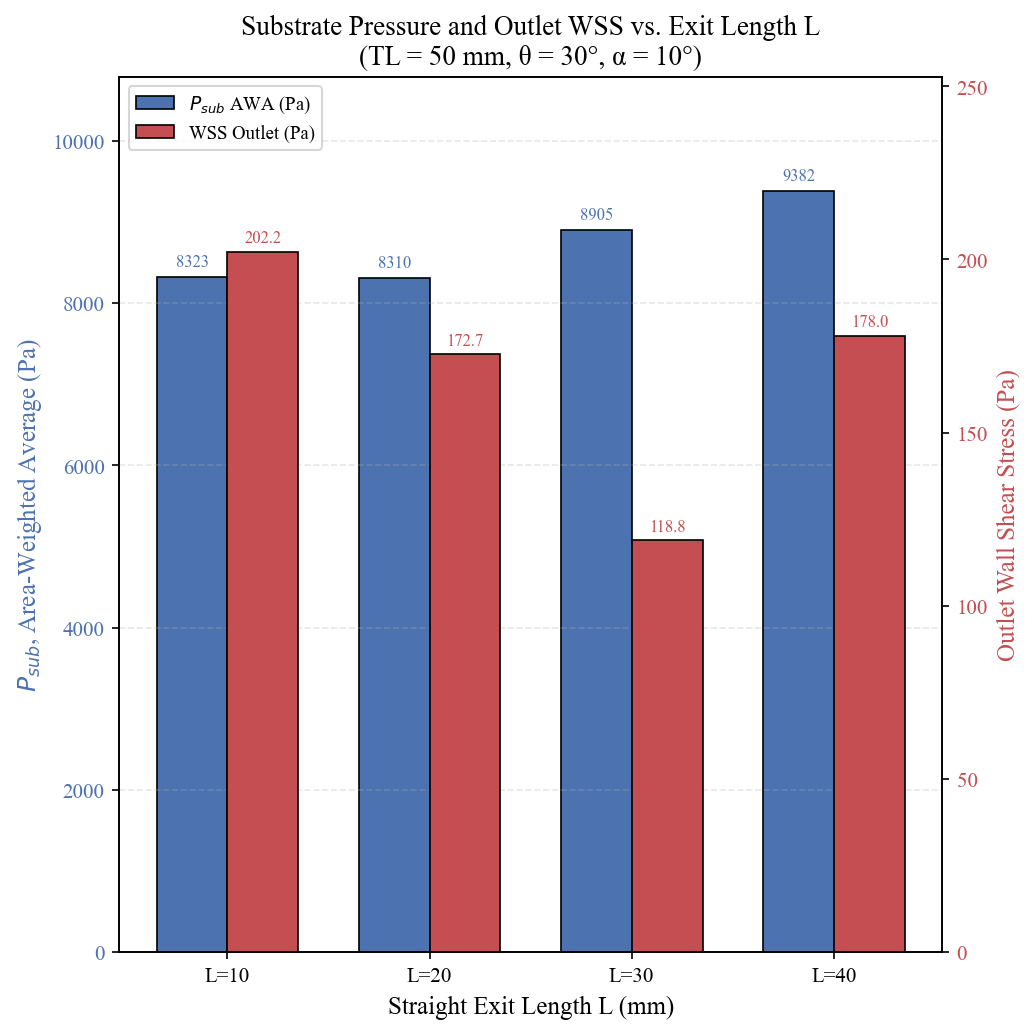
\includegraphics[width=0.8\textwidth]{figures/4.5.png}
  \caption{不同$L$下$P_{sub,AWA}$与$WSS_{outlet}$对比柱状图}
  \label{fig:4.5}
\end{figure}

由图可知，当高度$L$从10~mm增大至40~mm，$P_{sub,AWA}$从8323~Pa增至9382~Pa，增幅为+13\%。尽管变化趋势单调，但增幅相对有限，且数据点间的变化缺乏明显规律性，说明喷嘴收缩段竖向高度度对基底接触压力的调控能力较弱。

从物理机制来看，延长竖向高度主要增加了浆体在管道中的流动路程，对应更长的壁面摩擦损失路径，但由于出口面积不变，收缩段高度的增加不能像整形板那样通过改变流场几何形态来主动调控压力分布。收缩段高度的主要工程作用在于：为流体提供充分发展的速度剖面，确保进入整形板的流动状态稳定均匀。

$WSS_{outlet}$（整形板末端截面的壁面剪切应力）随$L$的变化呈现先降后升的非单调趋势，也反映了收缩段高度变化通过影响喷嘴出口速度剖面的充分发展程度，间接改变了整形板区域的局部流动状态。

总体来看，在本组对照试验的研究范围内（$L = 10$-40~mm），喷嘴收缩段竖向长度可视为对基底接触压力影响较小的次要参数，工程设计中可在满足制造约束的前提下灵活选取。

\section{整形板倾斜角$\alpha$的影响（B1组工况）}\label{sec:alpha-influence}

为研究整形板倾斜角度对喷嘴挤出性能的影响，本课题共选取5组工况进行了参数化研究。\cref{tab:4.4}总结了5组工况重点研究指标的结果。

\begin{table}[!htb]
  \centering
  \caption{B1组（$\alpha$变化）各工况评价指标汇总表}\label{tab:4.4}
  \renewcommand{\arraystretch}{1.3}
  \begin{tabular}{lcccccccc}
    \toprule
    \textbf{工况} & $\alpha$ & $H$(mm) & $P_{sub}$(Pa) & $WSS_{nozzle}$ & $\eta_p$ & $UI$ & $P_{inlet}$ \\
    \midrule
    B1-1     & 0°  & 22.00 & 5733  & 445.5 & 0.375 & 1.86 & 15274 \\
    B1-2     & 5°  & 17.64 & 6896  & 93.8  & 0.386 & 1.82 & 17856 \\
    Baseline & 10° & 13.32 & 8310  & 84.9  & 0.421 & 1.78 & 19750 \\
    B1-3     & 15° & 9.06  & 12081 & 77.1  & 0.481 & 1.64 & 25101 \\
    B1-4     & 20° & 4.90  & 22184 & 91.7  & 0.577 & 1.51 & 38418 \\
    \bottomrule
  \end{tabular}
\end{table}

\subsection{$\alpha$对基底压力的非线性影响}

\cref{fig:4.6}展示了$P_{sub,AWA}$随倾斜角$\alpha$变化的关系曲线，\cref{fig:4.7}和\cref{fig:4.8}分别展示了不同$\alpha$工况下的基底压力云图与速度流线对比。

\begin{figure}[!htb]
  \centering
  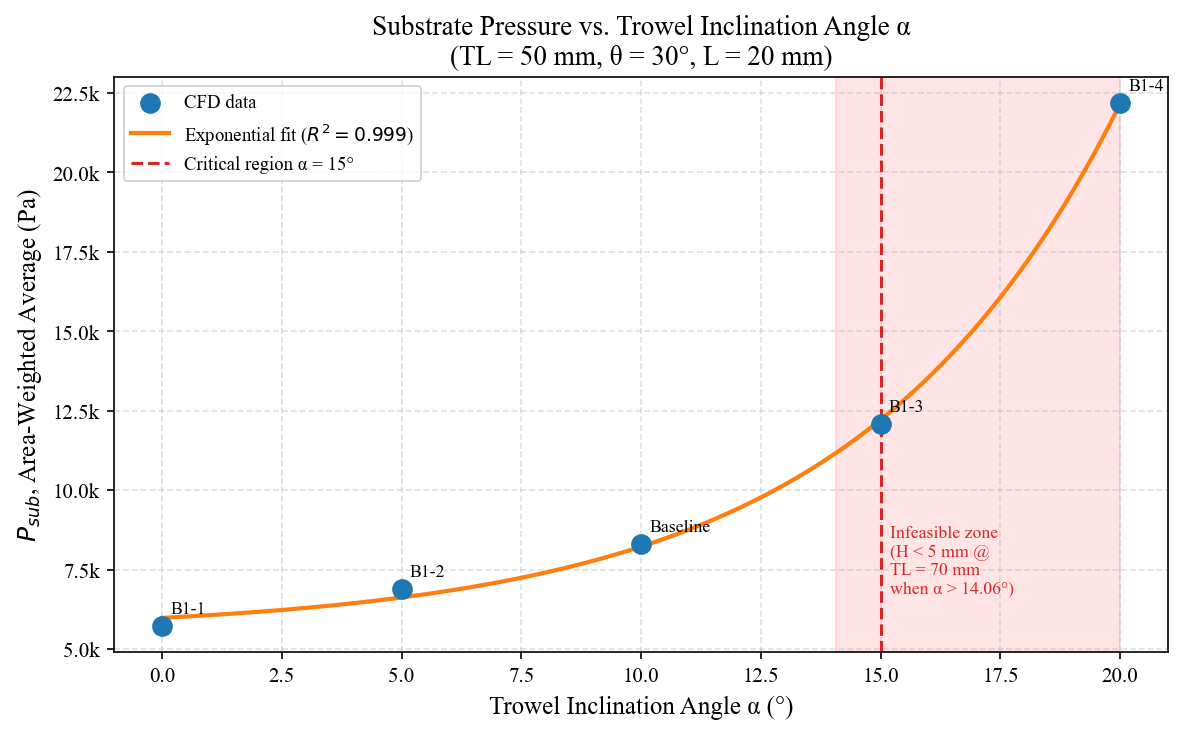
\includegraphics[width=0.75\textwidth]{figures/4.6.png}
  \caption{$P_{sub,AWA}$--$\alpha$关系曲线}
  \label{fig:4.6}
\end{figure}

\begin{figure}[!htb]
  \centering
  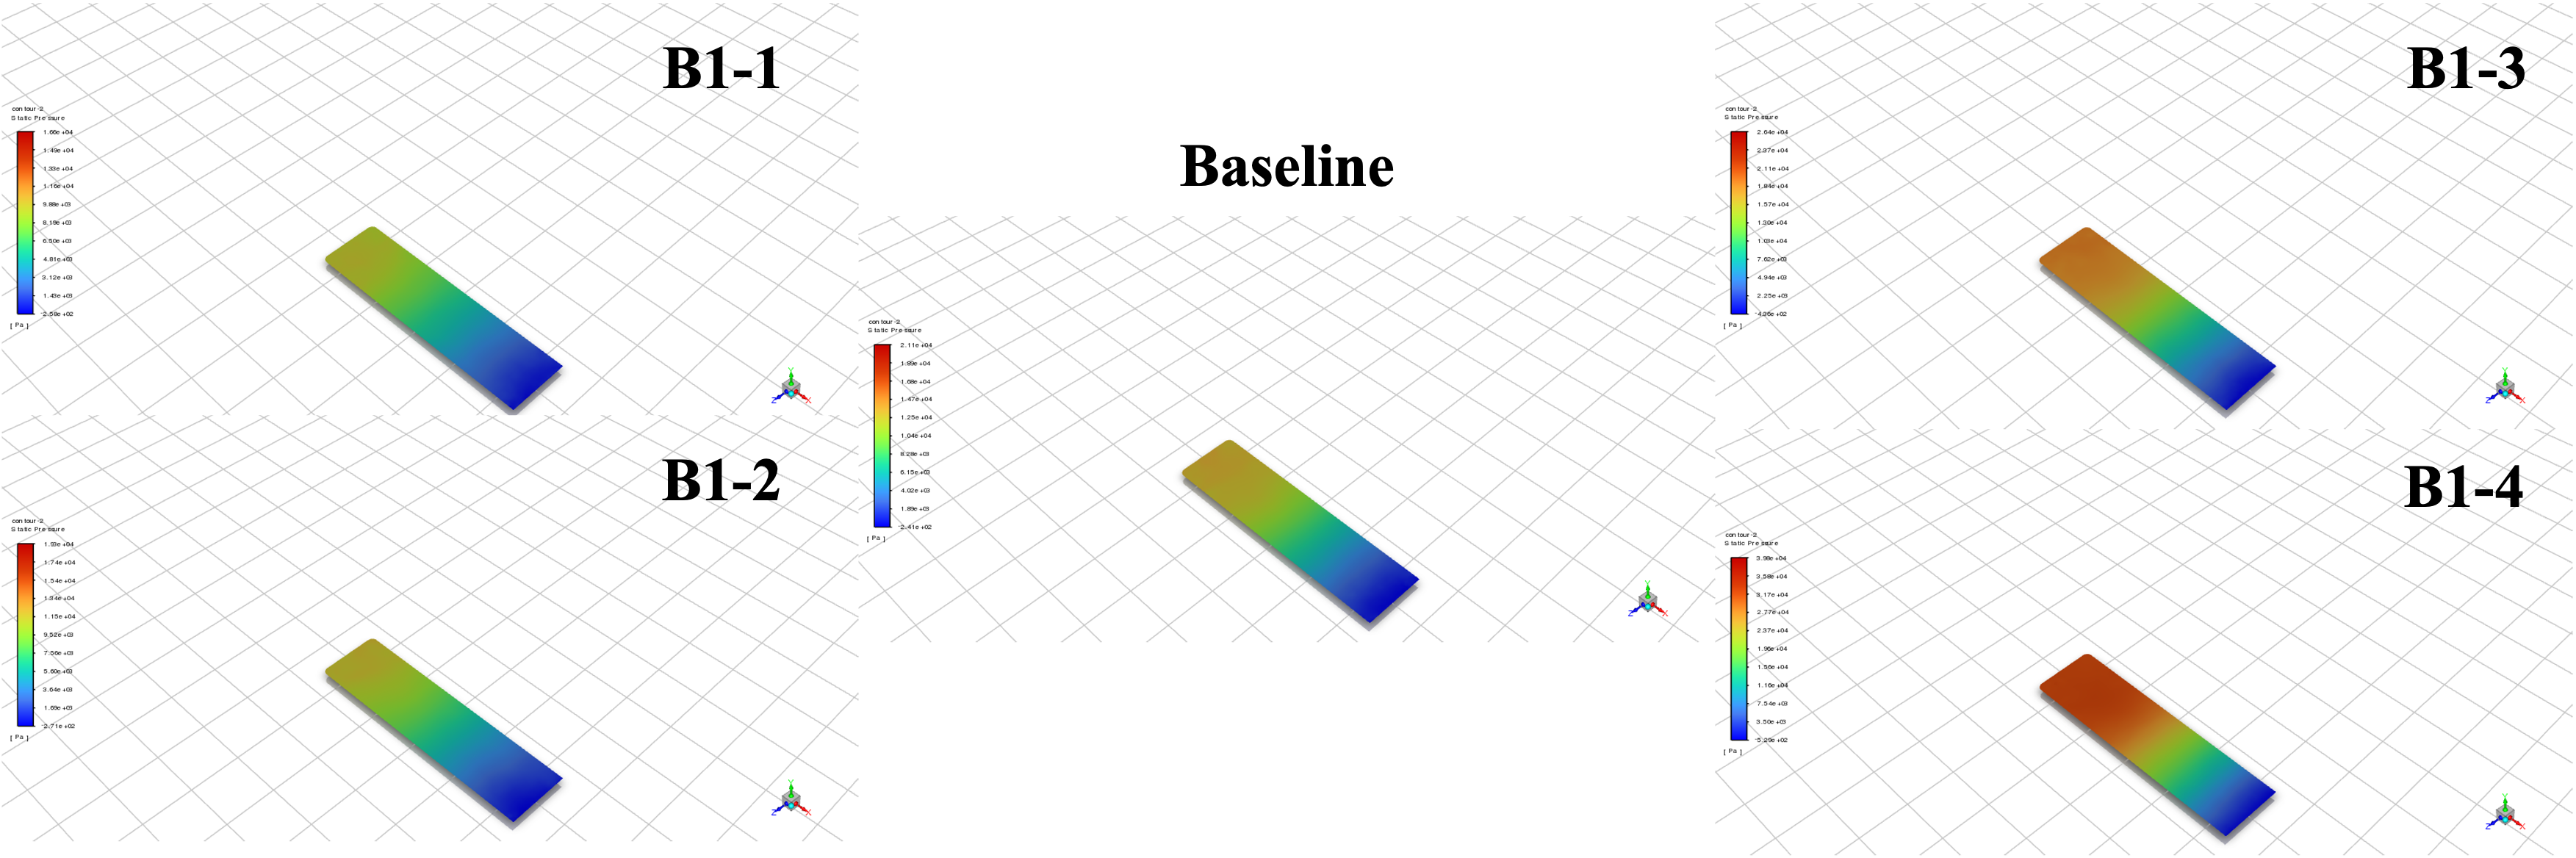
\includegraphics[width=0.9\textwidth]{figures/4.7.png}
  \caption{不同$\alpha$下基底压力云图对比图}
  \label{fig:4.7}
\end{figure}

\begin{figure}[!htb]
  \centering
  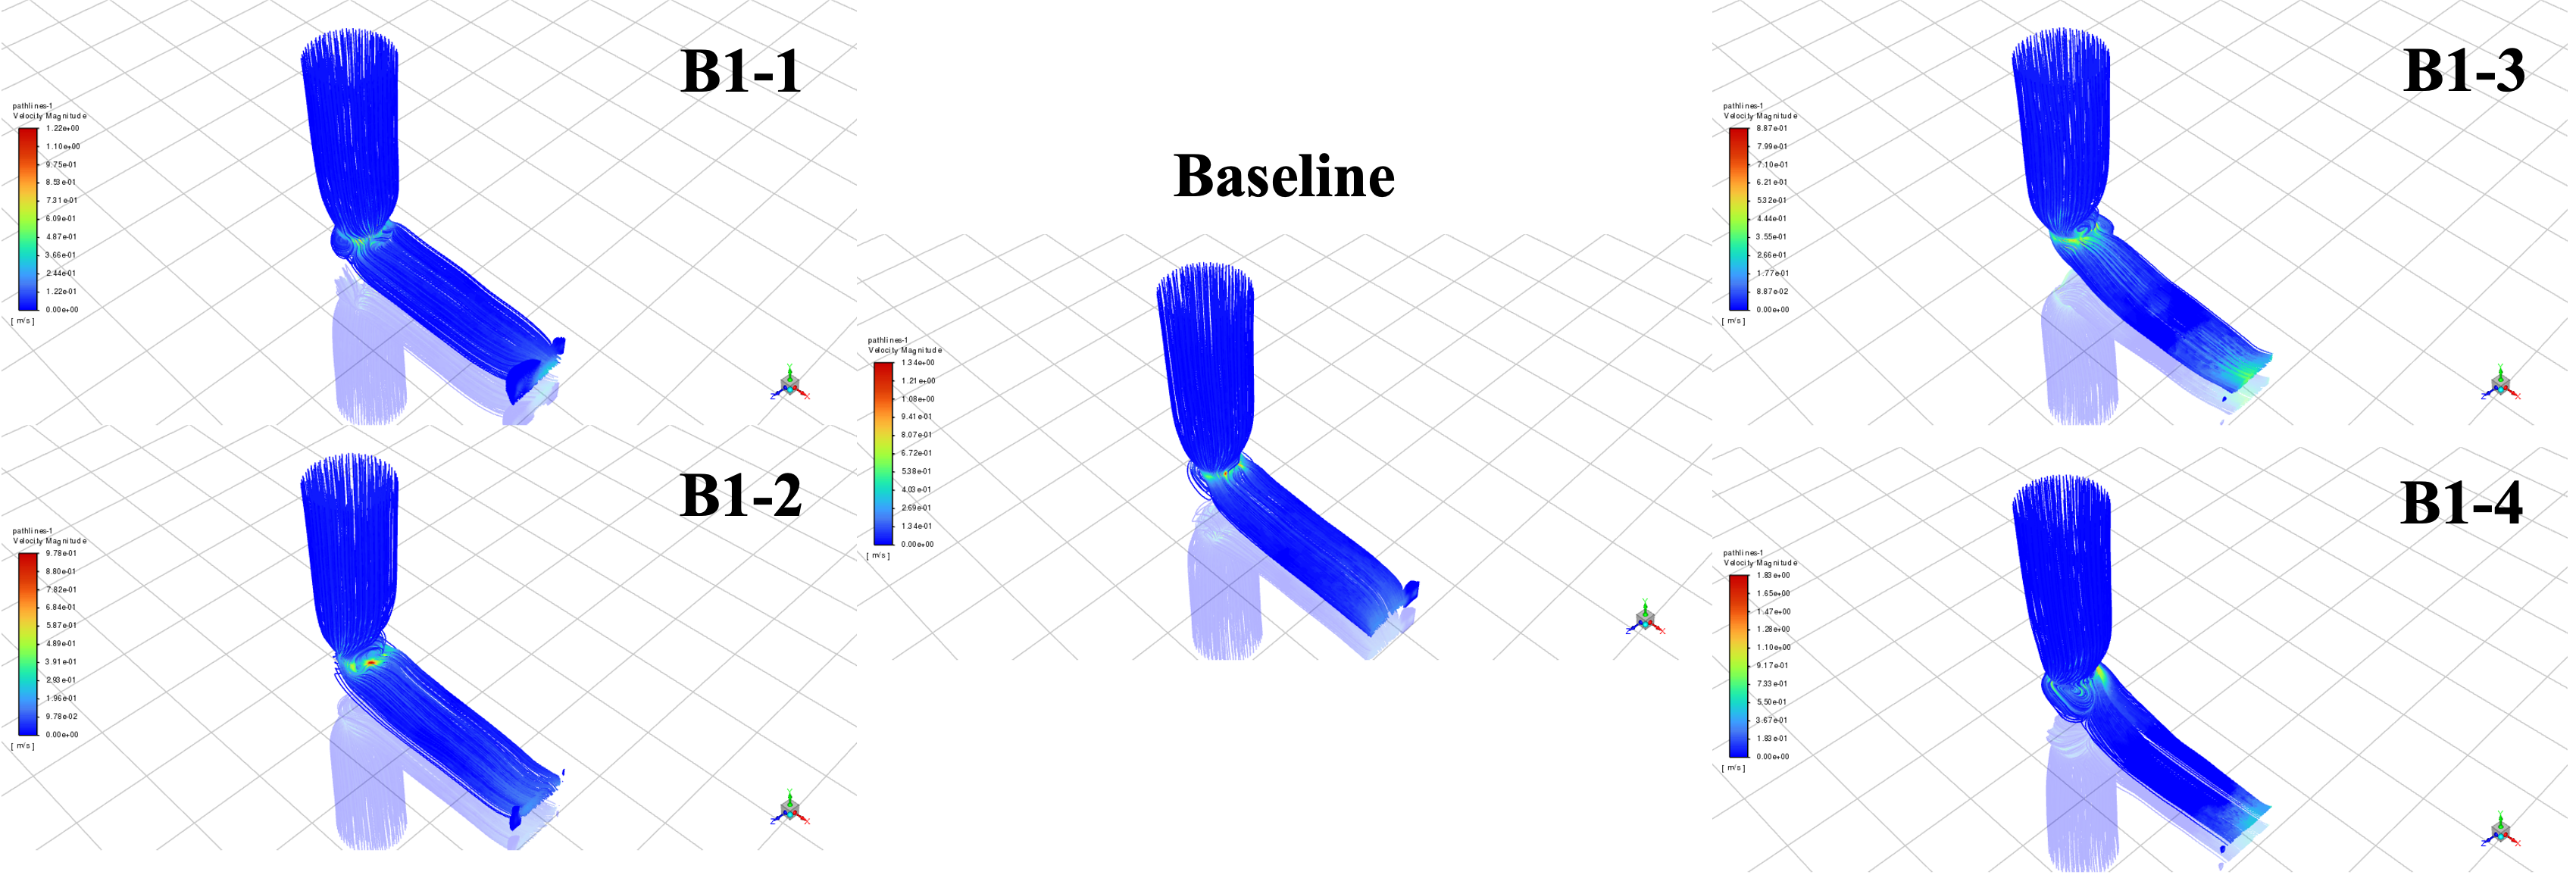
\includegraphics[width=0.9\textwidth]{figures/4.8.png}
  \caption{不同$\alpha$下速度流线对比图}
  \label{fig:4.8}
\end{figure}

结果表明，$\alpha$是本研究四个设计变量中对基底接触压力影响最为显著的参数。$\alpha$从0°增大至20°，$P_{sub,AWA}$从5733~Pa增至22184~Pa，增幅高达287\%。值得注意的是，该增长过程并非线性：在$\alpha \leq 15°$范围内，压力随$\alpha$的增大较为平稳；而在$\alpha$从15°增至20°时，压力出现非线性激增（12081~Pa$\to$22184~Pa，单步增幅+84\%），呈现明显的临界加速行为。

这一非线性现象的物理根源在于整形板出口处的楔形流动效应。由\cref{eq:H}给出的定量关系可知：随$\alpha$增大，整形板倾斜面与基底面之间形成的楔形通道出口间隙$H$（即层高）不断减小。在楔形受限流动中，压力增益与间隙高度的平方成反比，可由Reynolds楔形润滑方程近似描述，方程简化后形式为：
\begin{equation}\label{eq:wedge}
  \Delta P_{wedge} \approx \frac{6 \eta v \cdot L_{eff}}{h^2},
\end{equation}
其中$\eta$为浆体表观黏度，$v$为出料口流速，$L_{eff}$为楔形约束有效长度，$h$为出口间隙高度。由该式可见，当$h$减小时，$\Delta P_{wedge}$以$h^{-2}$的速率增大，间隙越小，压力增益越剧烈，这直接解释了$\alpha$从15°到20°时基底压力的非线性激增现象。

由\cref{eq:dH-dalpha}几何关系可知，层高$H$对$\alpha$的偏导数为$\partial H / \partial \alpha = -TL \cos(\alpha) < 0$，表明层高$H$随$\alpha$单调递减。随$\alpha$增大，楔形效应增强，基底压力迅速上升，但层高$H$同步减小，在$\alpha$超过可行性阈值后，沉积层过薄将无法保证打印质量，这构成了$\alpha$参数优化的核心约束，也说明整形板倾斜角的大小需要在保证打印层高度允许范围之内进行优化分析处理。

当$\alpha = 0°$时（工况B1-1），整形板出料段水平，不形成楔形约束，浆体在出料口处自由扩散，$WSS_{nozzle}$高达445.5~Pa，远超其他工况的5倍以上。这一异常高剪切应力源于$\alpha = 0°$时喷嘴出口流体在无约束条件下发生剧烈的方向转折，在前挡板附近产生强烈的回流涡和局部高速梯度区。

由于工况B1-1的截面壁面剪切应力数据偏离正常分布范围，将其纳入代理模型训练集会严重破坏模型的拟合质量，因此在后续的响应面建模中，B1-1并没有纳入相关模型的训练集，但其$P_{sub,AWA}$数据仍作为$\alpha = 0°$时的极限对照保留。

\subsection{$\alpha$与层高约束的解析关系}

层高约束$H \geq 5$~mm是本研究对$\alpha$参数设置的几何限制条件之一。由\cref{eq:H}反函数推导后，可得$\alpha$的可行上界：
\begin{equation}\label{eq:alpha-max}
  \alpha_{max} = \arcsin\left( \frac{Z_0 - H_{min}}{TL} \right).
\end{equation}
\cref{fig:4.9}展示了在$TL = 30, 40, 50, 60, 70$~mm五种整形板长度下，层高$H$随$\alpha$变化的曲线族。绿色区域（$H \geq 5$~mm）为几何可行域，红色区域（$H < 5$~mm）为不可行域。由图可见，当$TL$较大时，$\alpha$的可行范围更窄：$TL = 70$~mm时，$\alpha_{max} = \arcsin(17/70) = 14.06°$，而$TL = 30$~mm时，$\alpha_{max} = \arcsin(17/30) = 34.6°$。

B1-4工况（$\alpha = 20°$，$TL = 50$~mm）对应层高$H = 22 - 50 \times \sin(20°) = 4.90$~mm$< 5$~mm，不满足层高约束，虽然其$P_{sub,AWA} = 22184$~Pa为所有B1组工况最高，但因几何不可行而被排除出Pareto优化的可行域。在追求高接触压力的同时，层高约束是不可逾越的工程边界，优化设计必须在可行域内进行。

\begin{figure}[!htb]
  \centering
  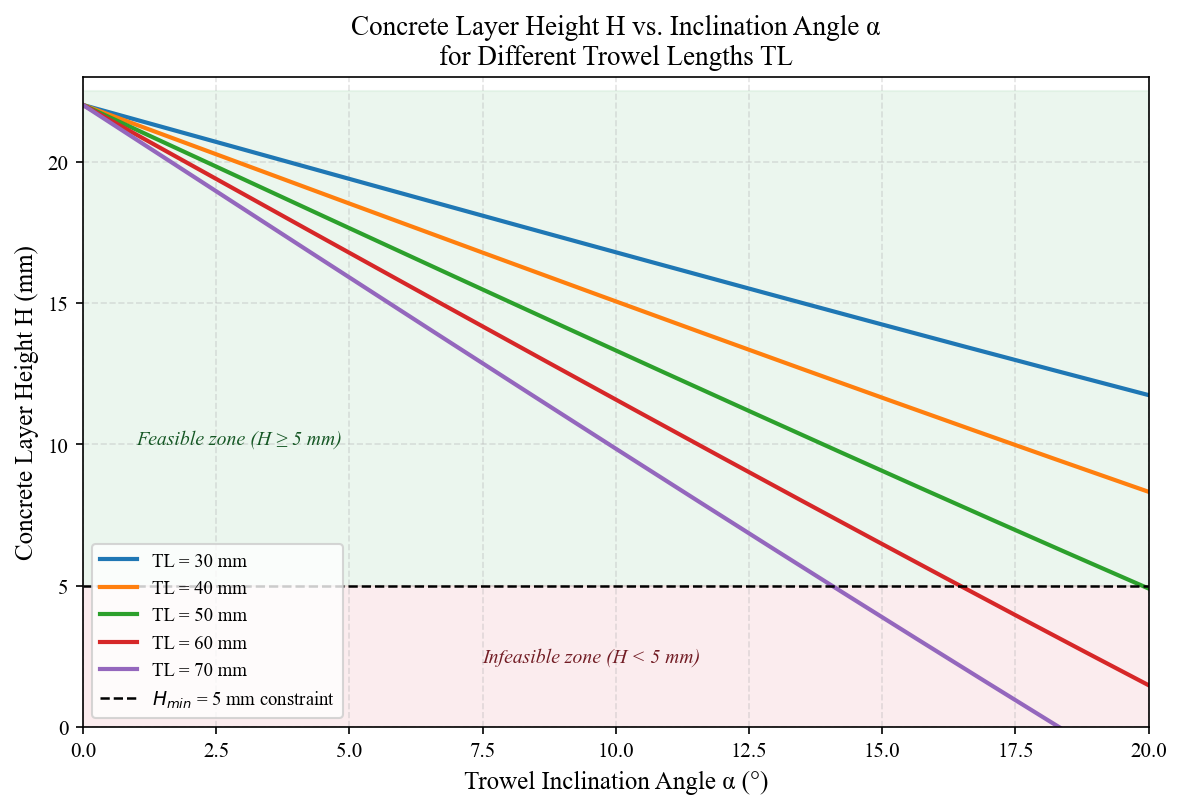
\includegraphics[width=0.8\textwidth]{figures/4.9.png}
  \caption{层高$H$与$\alpha$的关系图}
  \label{fig:4.9}
\end{figure}

\subsection{B1组工况综合评价}

综上所述，在满足层高约束的工况中，B1-3（$\alpha = 15°$）的综合性能最优：$P_{sub,AWA} = 12081$~Pa（较Baseline提升+45\%），$\eta_p = 0.481$（较Baseline提升+14\%），$UI = 1.64$（低于Baseline的1.78，压力均匀性改善）。尽管B1-3的$P_{inlet} = 25101$~Pa较Baseline高出27\%，但考虑到$P_{sub,AWA}$的大幅提升，压力传递效率的整体提高是值得的。B1-3的参数设置（$\alpha = 15°$）将在C组优化工况中被采用，与$\theta = 60°$的喷嘴参数组合，验证参数协同效应。

\section{整形板延伸长度$TL$的影响（B2组工况）}

为研究整形板延伸长度对喷嘴挤出性能的影响，本组研究固定整形板倾斜角为10°，共选取5组工况进行了参数化研究。\cref{tab:4.5}总结了5组工况重点研究指标的结果。\cref{fig:4.10}展示了$P_{sub,AWA}$随$TL$变化的折线图，\cref{fig:4.11}展示了五种$TL$工况下的基底压力云图对比，\cref{fig:4.12}展示了不同整形板延伸长度下基底面压力沿打印方向（X轴）分布曲线的叠加图。

\begin{table}[!htb]
  \centering
  \caption{B2组（$TL$变化）各工况评价指标汇总表}\label{tab:4.5}
  \renewcommand{\arraystretch}{1.3}
  \begin{tabular}{lcccccccc}
    \toprule
    \textbf{工况} & $TL$(mm) & $H$(mm) & $P_{sub}$(Pa) & $WSS_{nozzle}$ & $\eta_p$ & $UI$ & $P_{inlet}$ \\
    \midrule
    B2-1     & 30 & 16.79 & 5944  & 86.6  & 0.365 & 1.83 & 16277 \\
    B2-2     & 40 & 15.05 & 7177  & 81.0  & 0.390 & 1.79 & 18390 \\
    Baseline & 50 & 13.32 & 8310  & 84.9  & 0.421 & 1.78 & 19750 \\
    B2-3     & 60 & 11.58 & 10353 & 82.0  & 0.451 & 1.73 & 22937 \\
    B2-4     & 70 & 9.85  & 12833 & 102.1 & 0.483 & 1.68 & 26549 \\
    \bottomrule
  \end{tabular}
\end{table}

\begin{figure}[!htb]
  \centering
  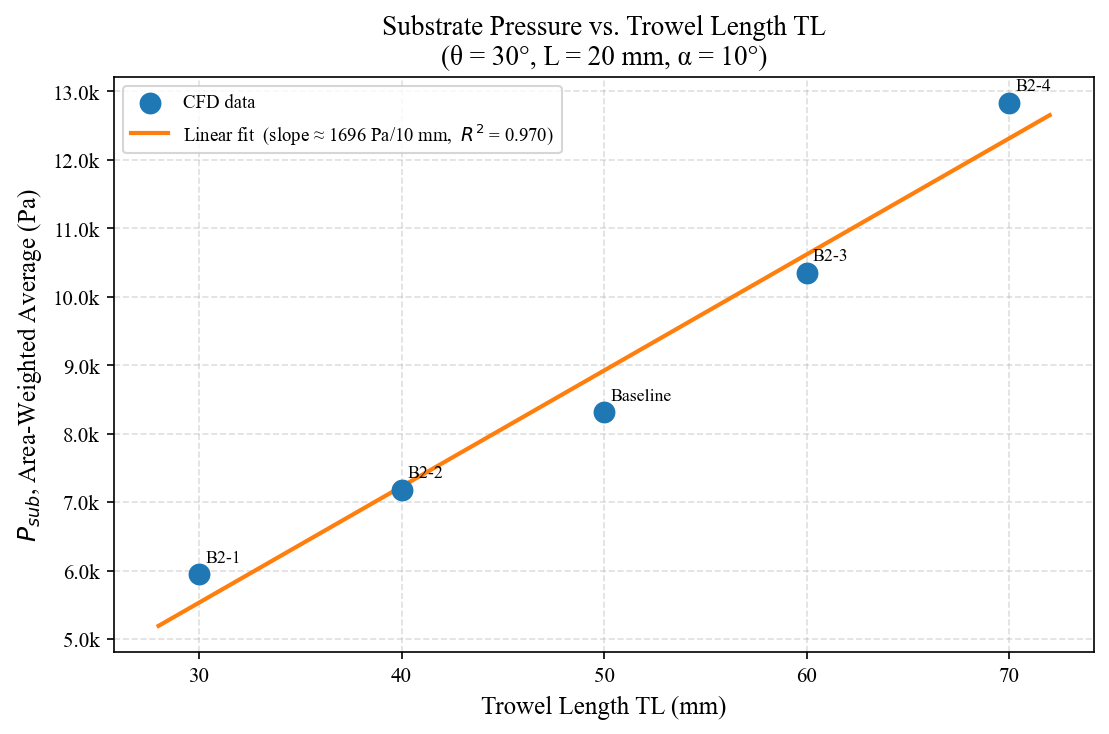
\includegraphics[width=0.75\textwidth]{figures/4.10.png}
  \caption{$P_{sub,AWA}$--$TL$折线图}
  \label{fig:4.10}
\end{figure}

\begin{figure}[!htb]
  \centering
  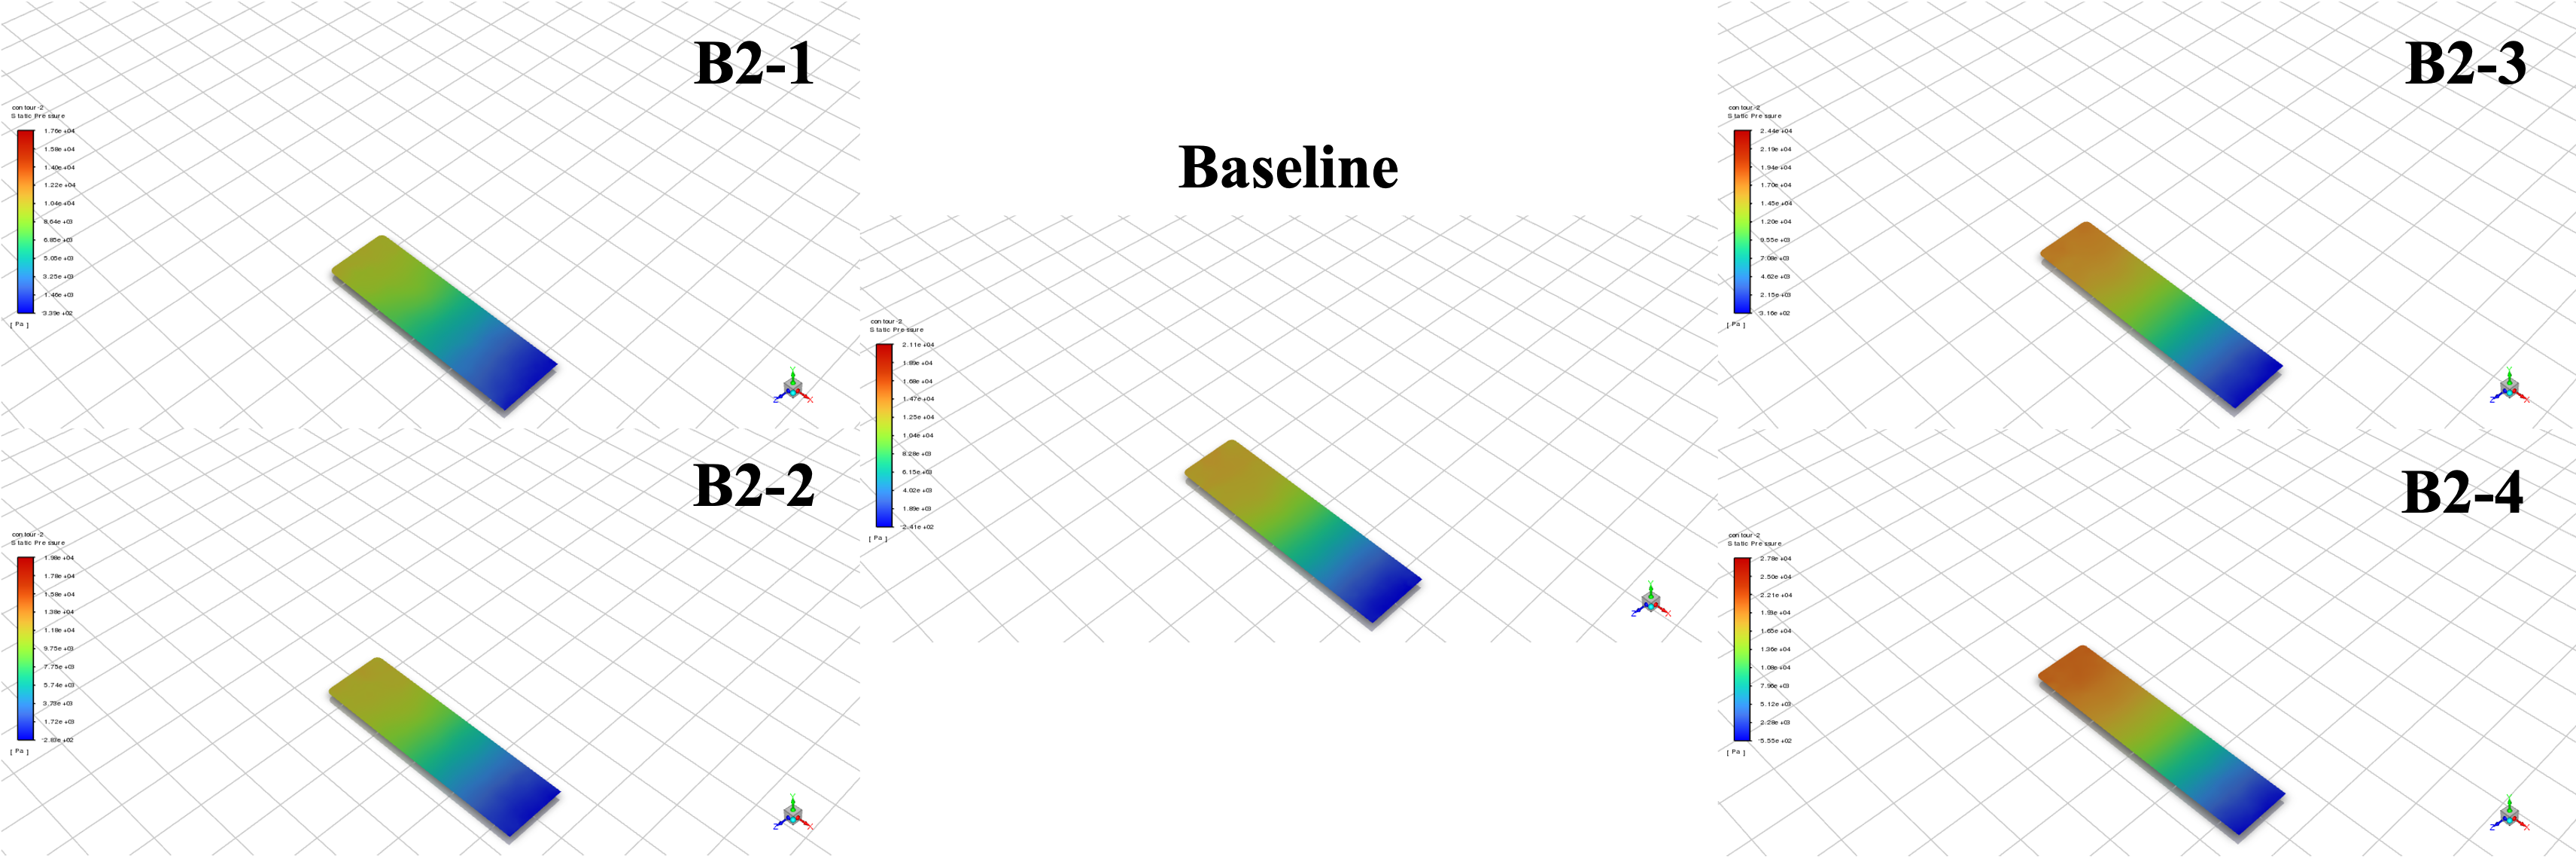
\includegraphics[width=0.9\textwidth]{figures/4.11.png}
  \caption{不同$TL$下基底压力云图对比图}
  \label{fig:4.11}
\end{figure}

\begin{figure}[!htb]
  \centering
  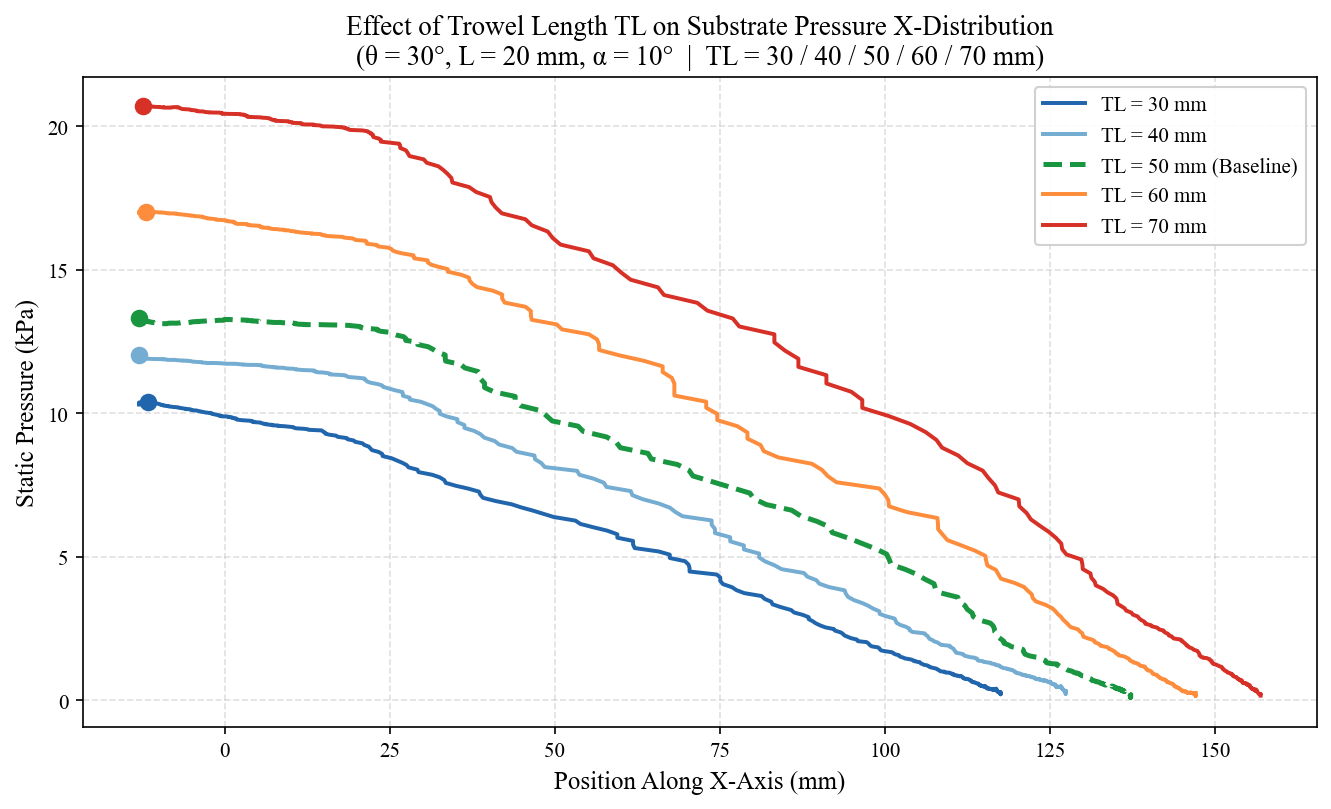
\includegraphics[width=0.8\textwidth]{figures/4.12.png}
  \caption{$TL$对基底压力XY分布曲线的影响图}
  \label{fig:4.12}
\end{figure}

由\cref{fig:4.10}可以看出，当$TL$从30~mm增大至70~mm，$P_{sub,AWA}$从5944~Pa增至12833~Pa，增幅为+116\%，Pearson相关系数$r = 0.541$（$p = 0.014$），具有统计显著性。线性拟合结果表明，$TL$每增加10~mm，$P_{sub,AWA}$约增加1700~Pa，两者近似呈线性正相关关系（$R^2 = 0.999$）。

从\cref{fig:4.12}的压力XY曲线叠加图中，可以清晰观察到整形板延伸长度影响的空间分布特征：随延伸长度增大，基底面压力的峰值不断升高，且高压区域沿打印方向（+X方向）的覆盖范围持续扩展，压力影响区域的范围随整形板的延伸而同步增大。这一空间扩展效应说明，$TL$的作用机制与$\alpha$有所不同：$\alpha$主要通过缩小出口间隙来增强楔形压力，而$TL$主要通过延长约束接触长度来积累压力。

从物理机理而言，更长的整形板提供了更长的流体约束路径，使浆体在受限空间内的停留时间更长，约束面对浆体施加压力的面积也更大，从而使总接触力显著提升。此外，由\cref{fig:4.12}还可得出：$TL$增大后整形板末端负压区的幅值略有增大，这是因为更长的整形板在末端产生更强的流动释放效应，局部分离更为明显。

与$\alpha$参数相比，$TL$是一种更为温和的增压手段。在相同的$P_{sub,AWA}$提升幅度下，通过增大$TL$所消耗的层高余量远小于通过增大$\alpha$：$TL = 70$~mm时层高仍有$H = 9.85$~mm（安全余量充足），而$\alpha = 15°$时层高已降至9.06~mm。因此，在工程实际中，优先通过增大$TL$来提升接触压力，以$\alpha$作为精细调节手段，是兼顾性能与安全余量的合理策略。

\section{优化工况组C分析}

\subsection{参数协同效应验证（C1组工况）}

基于研究线A和B的单因素分析结论，C1组工况通过将最优参数组合来探索参数间的协同增强效应。C1组共包含三组工况，其中C1-1与A1-4完全相同（$TL = 50$~mm，$\theta = 60°$，$\alpha = 10°$），代表A组工况下最大喷嘴收缩角带来的协同优化效应；C1-2（$TL = 55$~mm，$\theta = 30°$，$\alpha = 15°$）在保持喷嘴参数不变的条件下，仅对整形板参数进行优化，$P_{sub,AWA} = 14525$~Pa，较Baseline提升+75\%；C1-3（$TL = 60$~mm，$\theta = 60°$，$\alpha = 15°$）在C1-2的基础上同时将收缩角提升至$\theta = 60°$，$P_{sub,AWA} = 21677$~Pa，较Baseline提升+161\%。\cref{tab:4.6}总结了这三组工况的重点研究指标的结果，\cref{fig:4.13}展示了前四优化指标与基线水平的柱状对比图。

\begin{table}[!htb]
  \centering
  \caption{C1组（协同效应组）各工况评价指标汇总表}\label{tab:4.6}
  \renewcommand{\arraystretch}{1.3}
  \begin{tabular}{lcccccccc}
    \toprule
    \textbf{工况} & $TL$ & $\theta$ & $L$ & $\alpha$ & $P_{sub}$(Pa) & $WSS_{nozzle}$ & $\eta_p$ & $UI$ \\
    \midrule
    Baseline & 50 & 30 & 20 & 10 & 8310  & 84.9  & 0.421 & 1.78 \\
    C1-1     & 50 & 60 & 20 & 10 & 9926  & 35.00 & 0.447 & 1.84 \\
    C1-2     & 55 & 30 & 20 & 15 & 14525 & 74.66 & 0.506 & 1.64 \\
    C1-3     & 60 & 60 & 20 & 15 & 21677 & 41.07 & 0.557 & 1.58 \\
    \bottomrule
  \end{tabular}
\end{table}

\begin{figure}[!htb]
  \centering
  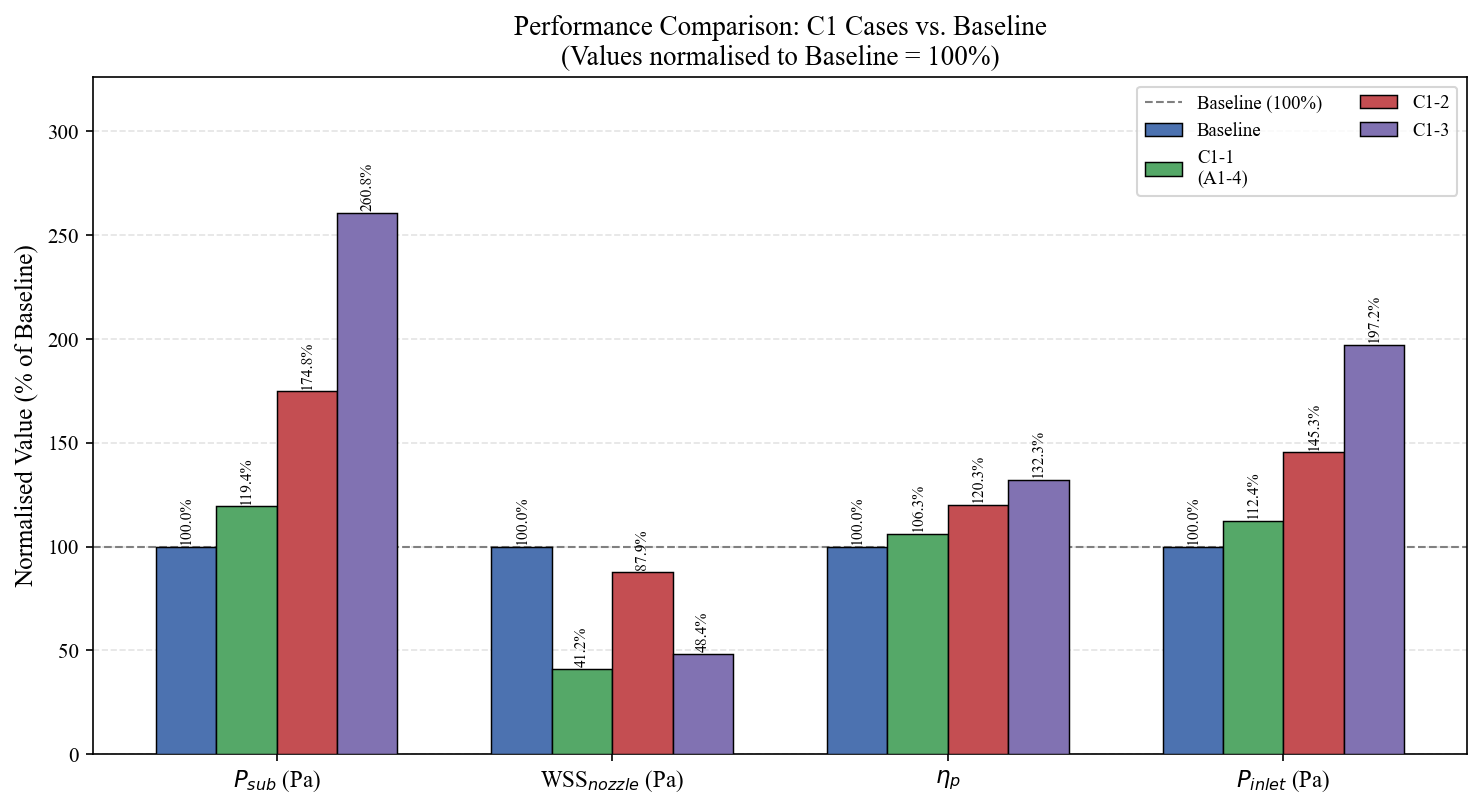
\includegraphics[width=0.85\textwidth]{figures/4.13.png}
  \caption{C1组别四优化指标与基线水平的柱状对比图}
  \label{fig:4.13}
\end{figure}

值得重点关注的是，C1-3的提升幅度（+161\%）显著超过了A1-4（仅优化$\theta$，+19\%）与C1-2（仅优化整形板，+75\%）两者效果的简单叠加（+94\%）。这一效应表明，喷嘴收缩角$\theta = 60°$与整形板参数$\alpha = 15°$、$TL = 60$~mm之间存在正向协同放大机制：大收缩角使喷嘴出口流体具有更高的动压和更均匀的速度剖面，当这一高动压流体进入由较大$\alpha$和较长$TL$所形成的强楔形约束空间时，楔形效应对高动压流体的压力转化效率更高，两种效应相互增强，产生超线性的压力增益。\cref{fig:4.14}中的基底压力XY分布叠加曲线直观展示了这一协同效应：C1-3（$\theta = 60°$，$\alpha = 15°$）的压力分布曲线不仅峰值最高，覆盖范围也最广，明显优于同$\alpha$但$\theta = 30°$的B1-3工况。

\begin{figure}[!htb]
  \centering
  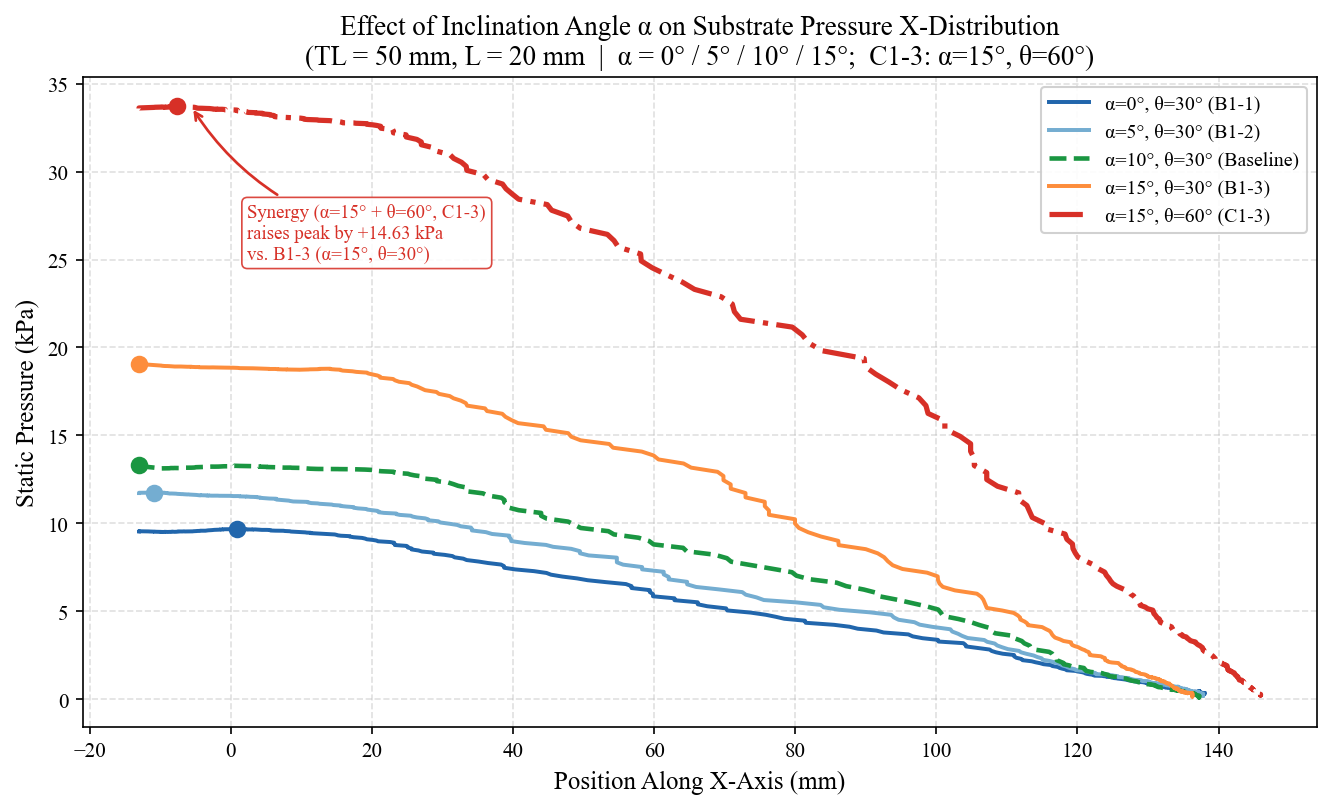
\includegraphics[width=0.8\textwidth]{figures/4.14.png}
  \caption{不同参数组合下基底面压力XY分布曲线叠加图}
  \label{fig:4.14}
\end{figure}

\subsection{无顶板整形板对照分析（C2工况）}

C2组工况作为对比试验验证整形板这一元件对混凝土打印浆体基础的正向效应。C2工况去除了整形板顶板，仅保留前挡板与75~mm延伸段，整形板出口平面已不存在，定义在喷嘴出口平面+X向坐标最大点处切线所在的ZY平面上；压力释放口仍然定义在延伸段出口所在平面。\cref{tab:4.7}总结了C2工况与基础工况的重点研究指标结果对比。结果表明，C2工况的$P_{sub,AWA} = 3436$~Pa，为全部20个工况中最低，较Baseline大幅降低59\%。

\begin{table}[!htb]
  \centering
  \caption{C2工况评价指标对比表}\label{tab:4.7}
  \renewcommand{\arraystretch}{1.3}
  \begin{tabular}{lcccccccc}
    \toprule
    \textbf{工况} & $TL$ & $\theta$ & $L$ & $\alpha$ & $P_{sub}$(Pa) & $WSS_{nozzle}$ & $\eta_p$ & $UI$ \\
    \midrule
    Baseline & 50  & 30 & 20 & 10 & 8310 & 84.9 & 0.421 & 1.78 \\
    C2       & --- & 30 & 20 & ---& 3436 & 382  & 0.300 & 2.09 \\
    \bottomrule
  \end{tabular}
\end{table}

\begin{figure}[!htb]
  \centering
  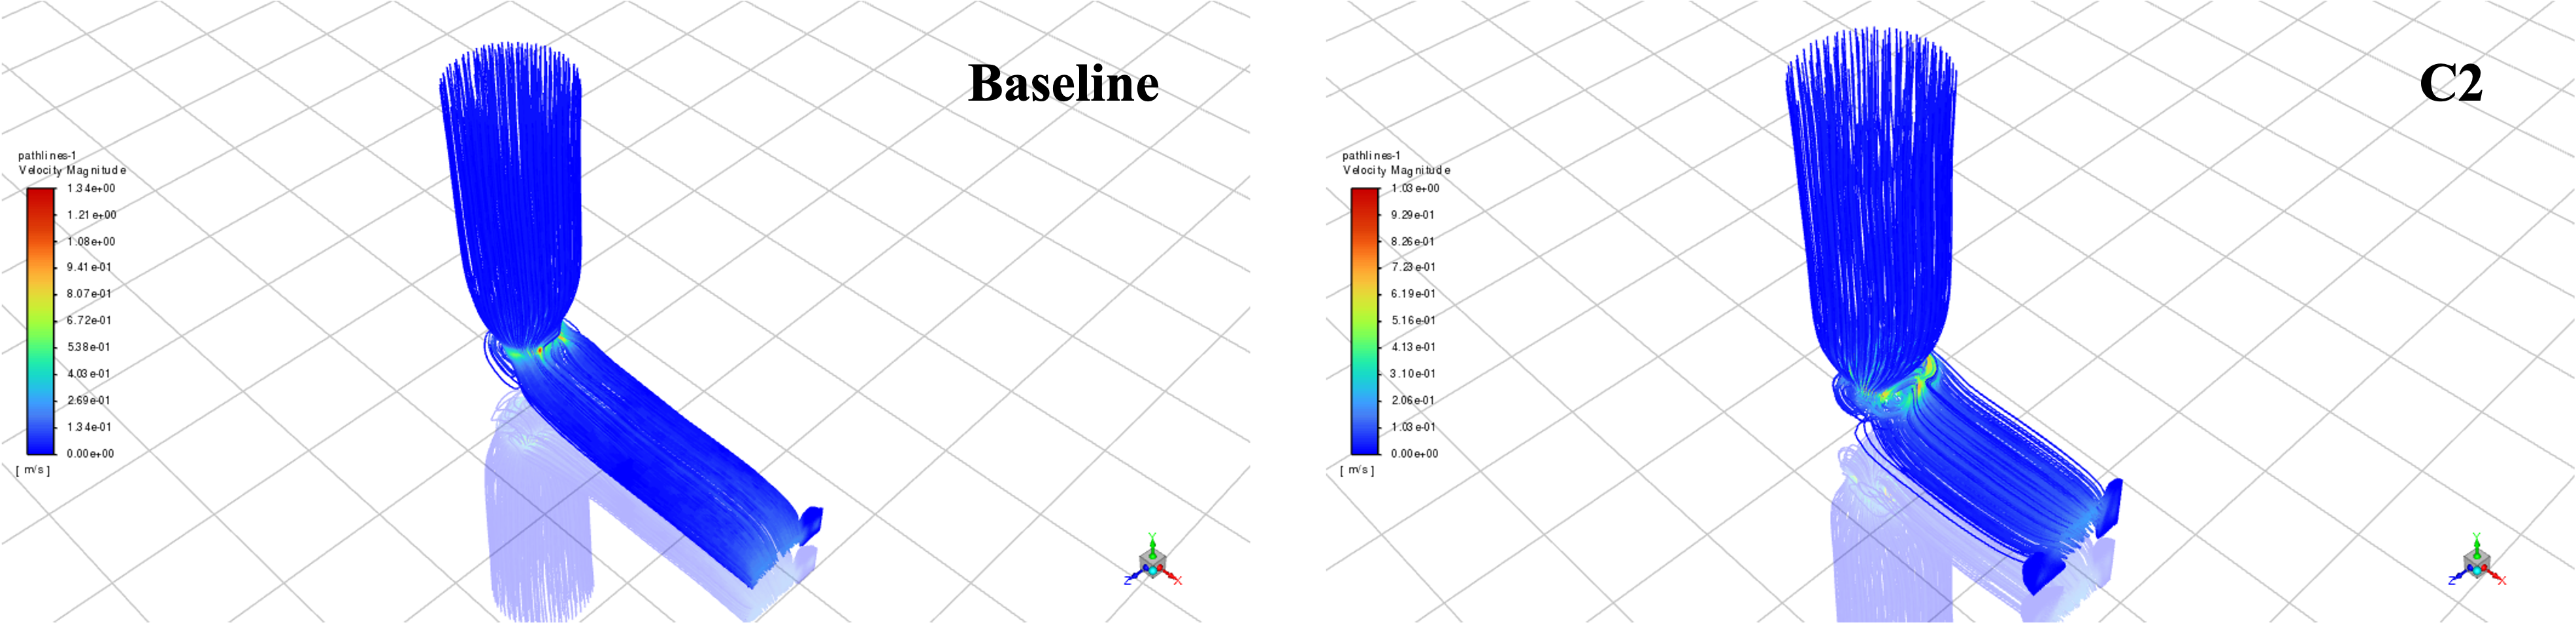
\includegraphics[width=0.9\textwidth]{figures/4.15.png}
  \caption{C2与基线工况的速度流线对比}
  \label{fig:4.15}
\end{figure}

\cref{fig:4.15}将C2与Baseline的速度场进行了对比。在Baseline工况中，顶板的存在对浆体形成封闭约束，使流体无法向上方逸散，所有动能被强制导向基底方向，形成有效的接触压力；而在C2工况中，去除顶板后流体可向上方自由扩散，约束空间开放，浆体的大部分动能以扩散流动的形式耗散，无法有效转化为对基底面的静压力，导致接触压力大幅降低。

C2工况还呈现出一个值得关注的特殊现象：整形转向后出口处的面积加权平均压力（8563~Pa）高于喷嘴平面处（3562~Pa），表现出沿流动方向的非单调压力分布特征。该现象的产生可能与C2工况下流场结构的显著变化密切相关。在去除顶板后，出口区域失去了原有的上壁约束，浆体在离开喷嘴后发生明显的自由扩散。由于流体向两侧扩张，出口截面附近局部区域出现低速滞留甚至回流现象，并伴随局部低压区形成，最小静压达到$-302$~Pa。这些低压区域在面积加权平均过程中显著拉低了喷嘴平面处的平均压力值。相比之下，整形转向后真实出口区域仍受到前挡板的局部约束作用，流体横向扩散受到抑制，局部流体减速并产生一定程度的压力积聚，因此其面积加权平均压力反而高于喷嘴平面处。这个结果并不违反流体力学规律，而是无顶板工况下自由扩散、局部回流以及约束条件变化共同作用的结果。这也说明，在存在明显流场分离与扩散结构的工况下，传统基于截面平均压力的比较方法需要结合具体流场形态进行综合分析。

C2工况的分析证明：整形板顶板是产生有效基底接触压力的核心结构，其封闭约束作用不可或缺。在实际打印系统设计中，整形板顶板的存在是提升层间粘结性能的必要条件。

\subsection{拓扑几何优化分析（C3工况）}

C3工况在C1-3几何参数（$TL = 60$~mm，$\theta = 60°$，$L = 20$~mm，$\alpha = 15°$）基础上，对喷嘴收缩段与直管段的转角处、整形板各转角处进行3-5~mm的圆角过渡处理（Fillet），以探究几何倒角对流场特性的影响。\cref{tab:4.8}总结了C3工况与基础工况的重点研究指标结果对比。

\begin{table}[!htb]
  \centering
  \caption{C3工况评价指标对比表}\label{tab:4.8}
  \renewcommand{\arraystretch}{1.3}
  \begin{tabular}{lcccccccc}
    \toprule
    \textbf{工况} & $TL$ & $\theta$ & $L$ & $\alpha$ & $P_{sub}$(Pa) & $WSS_{nozzle}$ & $\eta_p$ & $UI$ \\
    \midrule
    Baseline & 50 & 30 & 20 & 10 & 8310  & 84.9  & 0.421 & 1.78 \\
    C3       & 60 & 60 & 20 & 15 & 21702 & 25.13 & 0.560 & 1.58 \\
    \bottomrule
  \end{tabular}
\end{table}

压力结果方面，C3的$P_{sub,AWA} = 21702$~Pa，与C1-3的21677~Pa相差不足0.1\%，差异可忽略。这一结果说明，转角处的几何倒角对整体压力场的宏观分布影响极为有限。这说明基底接触压力主要由流道的宏观收缩比（由$\theta$决定）和整形板的楔形约束几何（由$\alpha$和$TL$决定）所主导，局部转角的圆化处理不改变这两个主控因素，因此对压力场的影响在工程精度范围内可视为零。

然而，剪切应力结果却呈现出显著的差异：C3的$WSS_{nozzle} = 25.1$~Pa，较C1-3的41.1~Pa降低了39\%。倒角消除了收缩段与直管段转角处的几何尖角，流线在此区域得以平滑过渡，避免了尖角处流动分离导致的局部高速梯度集中，在流场上表现为高剪切速率区被显著抑制，近壁速度梯度分布更为均匀，因而壁面剪切应力大幅降低。

综合而言，C3工况以几乎不损失接触压力性能（$\Delta P_{sub} < 0.1\%$）为代价，实现了$WSS_{nozzle}$ 39\%的显著改善，是本课题研究工况中最佳的几何构型。倒角设计作为一种低成本的几何优化手段，在实际打印喷嘴制造中值得推广应用。

\cref{fig:4.16}总结了C3工况的完整流场速度、压力、壁面剪切应力展示图；\cref{fig:4.17}展示了C3与Baseline工况五项指标归一化后的雷达图对比，直观展示了C3在各维度的综合优越性。

\begin{figure}[!htb]
  \centering
  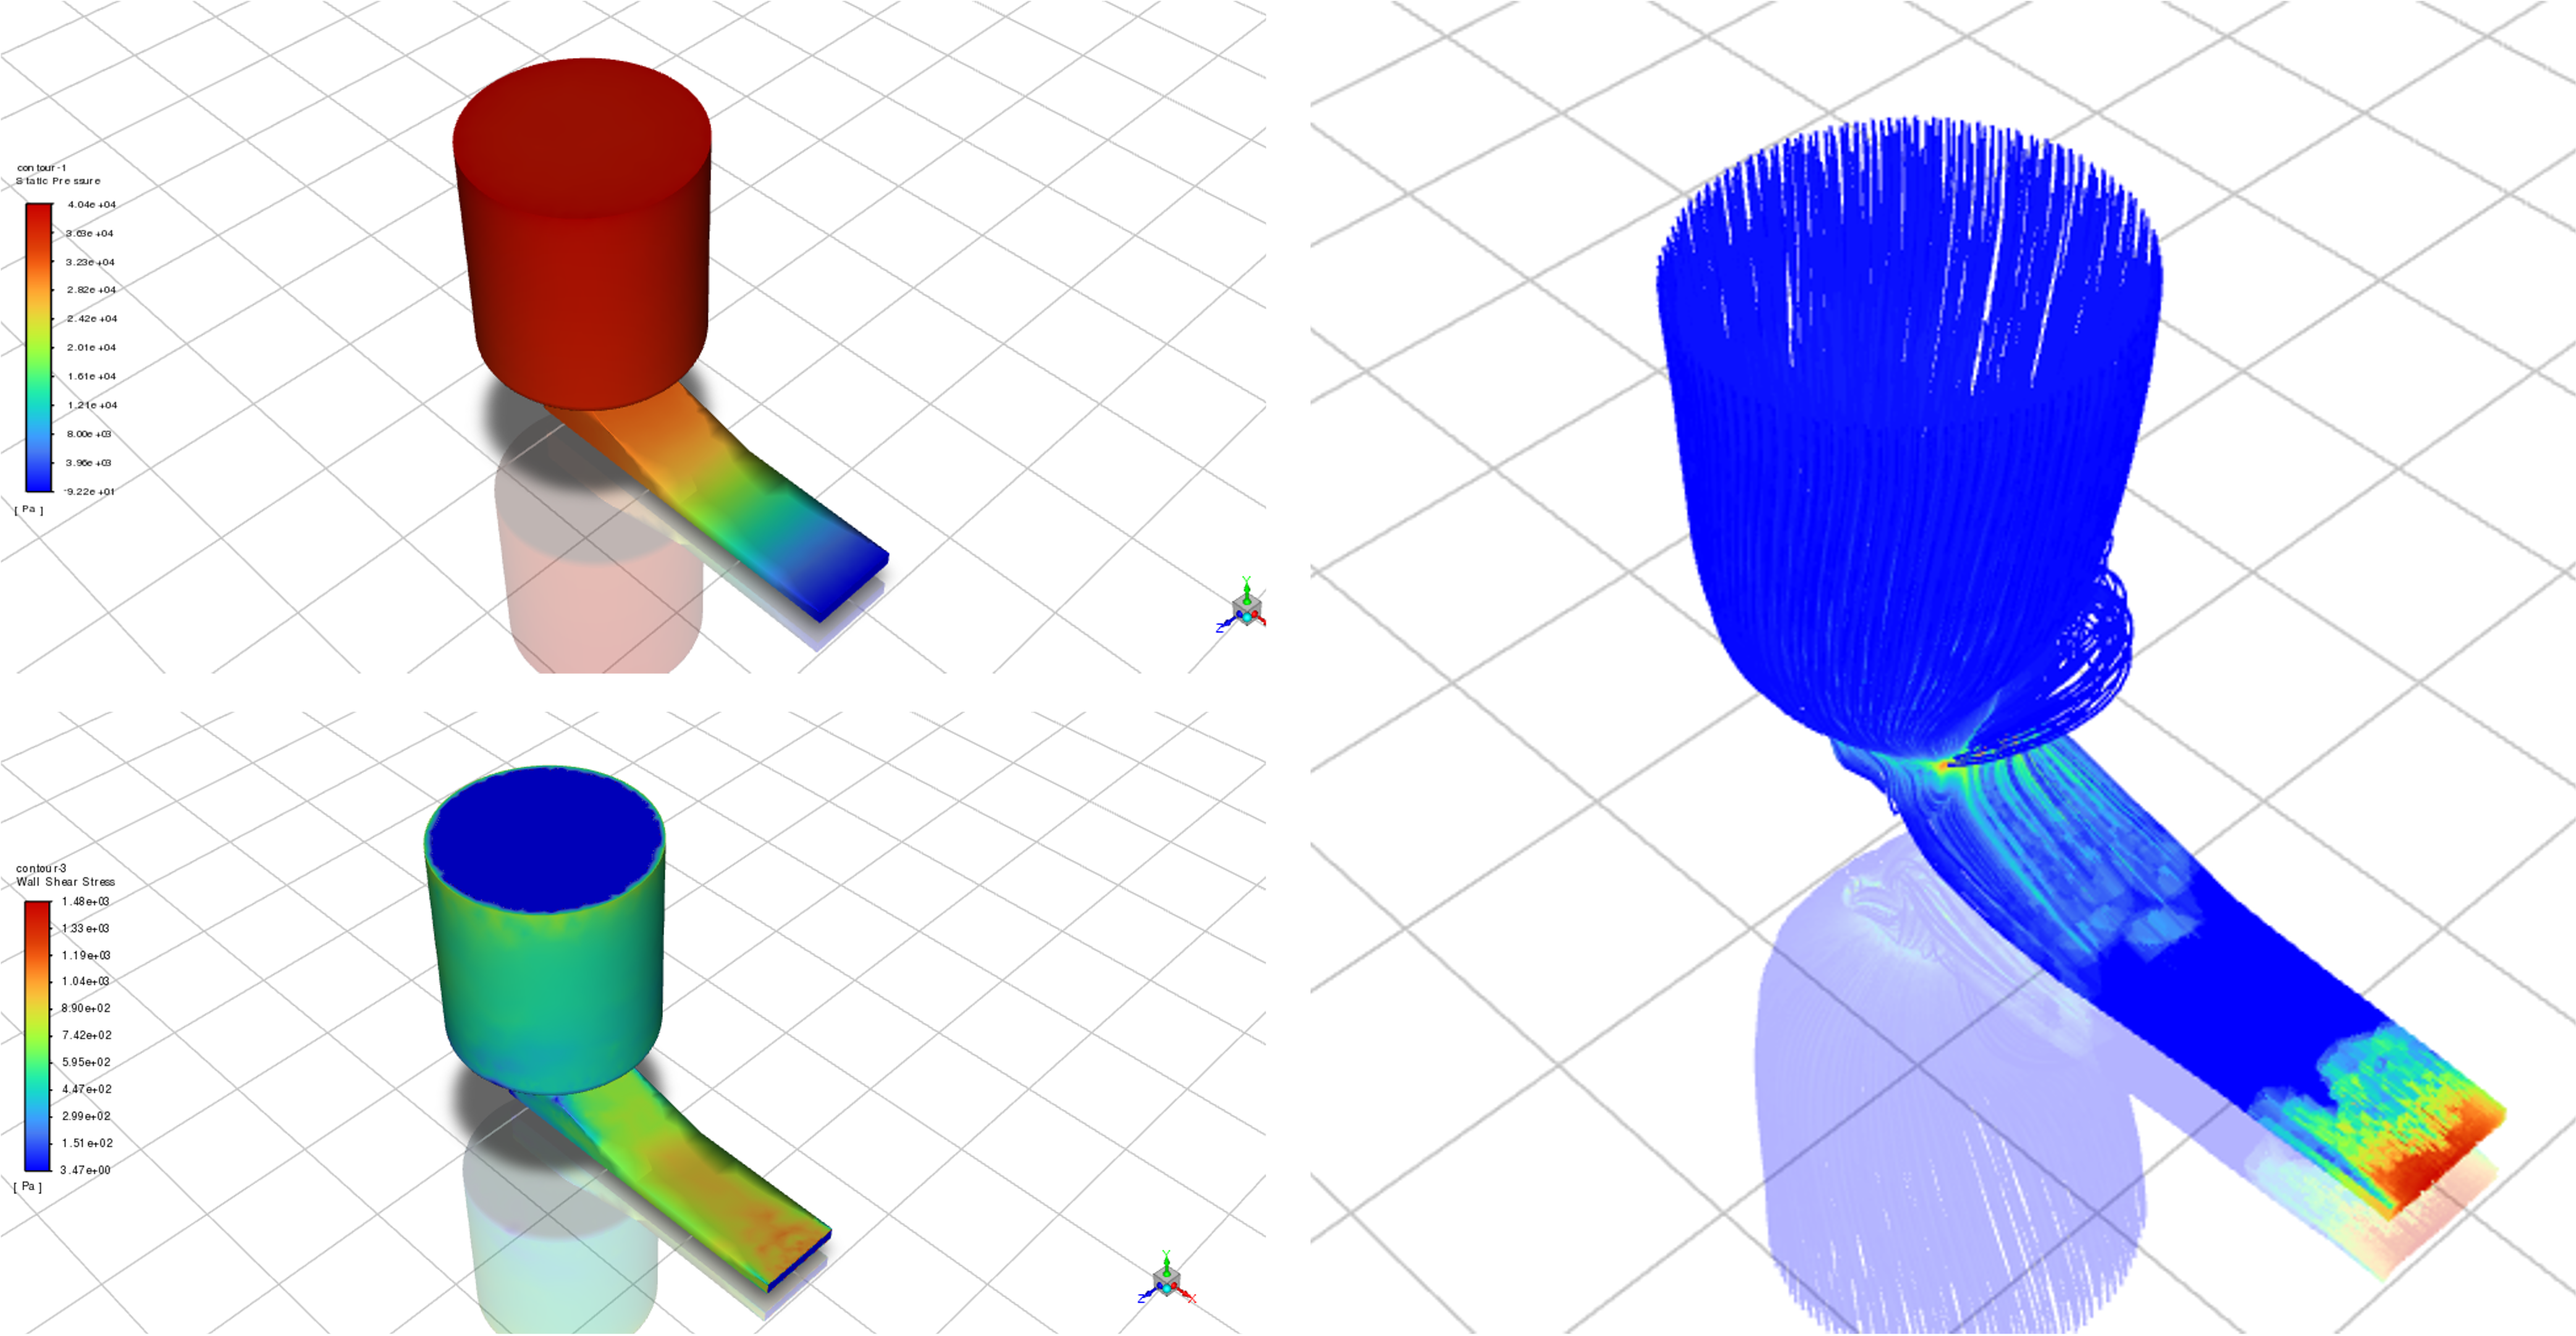
\includegraphics[width=0.9\textwidth]{figures/4.16.png}
  \caption{C3工况流场速度、压力、壁面剪切应力图}
  \label{fig:4.16}
\end{figure}

\begin{figure}[!htb]
  \centering
  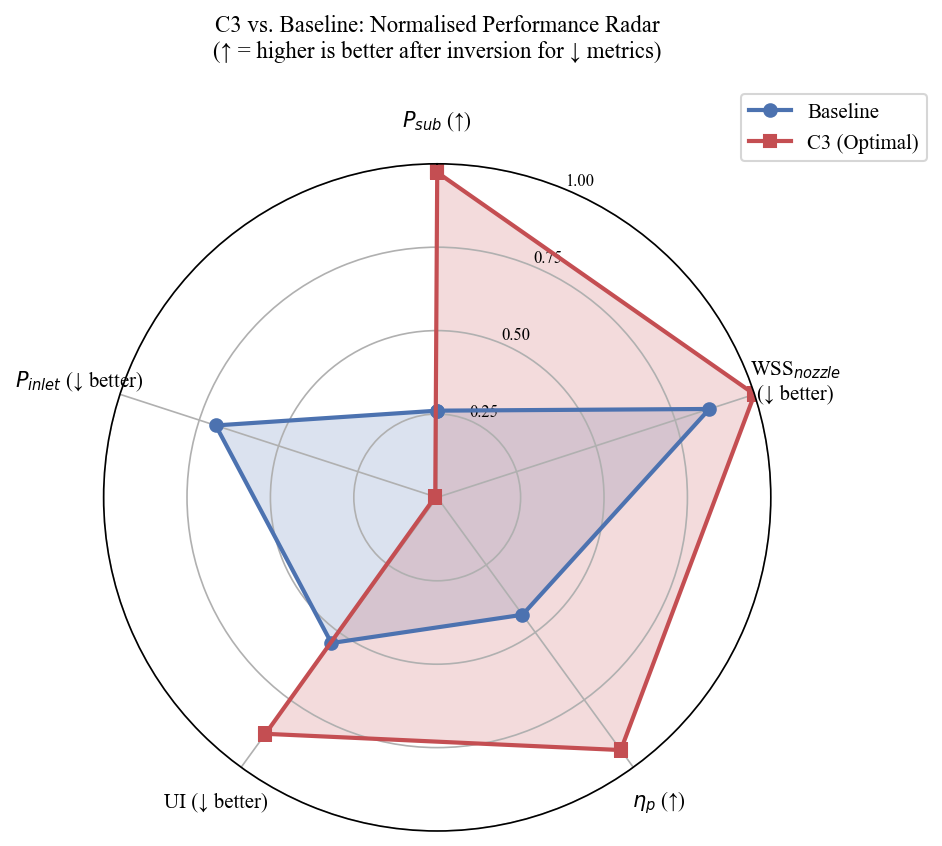
\includegraphics[width=0.7\textwidth]{figures/4.17.png}
  \caption{C3工况与基线工况对比雷达图}
  \label{fig:4.17}
\end{figure}

\section{参数影响规律综合对比}

\subsection{代表性工况数据汇总表}

\cref{tab:4.9}列举了代表性工况的完整评价指标。从对照工况C2（无顶板，$P_{sub} = 3436$~Pa）到最优工况C3（$P_{sub} = 21702$~Pa），基底接触压力跨越了约6倍的范围，说明喷嘴与整形板的几何设计对打印层间粘结性能具有决定性影响，远超材料流变参数微调所能带来的效益。

\begin{table}[!htb]
  \centering
  \caption{代表性工况评价指标汇总表}\label{tab:4.9}
  \renewcommand{\arraystretch}{1.3}
  \footnotesize
  \begin{tabular}{lcccccccccc}
    \toprule
    \textbf{工况} & $\theta$ & $L$ & $TL$ & $\alpha$ & $P_{sub,AWA}$ & $P_{sub,Max}$ & $WSS_{nozzle}$ & $\eta_p$ & $UI$ \\
    \midrule
    Baseline & 30° & 20 & 50 & 10° & 8310  & 13983 & 84.9  & 0.421 & 1.776 \\
    A1-4     & 60° & 20 & 50 & 10° & 9926  & 17858 & 35.0  & 0.447 & 1.842 \\
    B1-3     & 30° & 20 & 50 & 15° & 12081 & 19501 & 77.1  & 0.481 & 1.645 \\
    B2-4     & 30° & 20 & 70 & 10° & 12833 & 21089 & 102.1 & 0.483 & 1.683 \\
    C2       & 30° & 20 & 0  & 10° & 3436  & 6238  & 382.2 & 0.300 & 2.087 \\
    C3       & 60° & 20 & 60 & 15° & 21702 & 34234 & 25.1  & 0.560 & 1.582 \\
    \bottomrule
  \end{tabular}
\end{table}

\subsection{各参数影响幅度定量对比}

基于各研究线的单因素极差分析，四个设计变量对$P_{sub,AWA}$的影响幅度排序为：
\begin{equation}\label{eq:rank}
  \alpha\ (198\%) > TL\ (82.9\%) \gg \theta\ (19.7\%) > L\ (12.8\%).
\end{equation}

\begin{figure}[!htb]
  \centering
  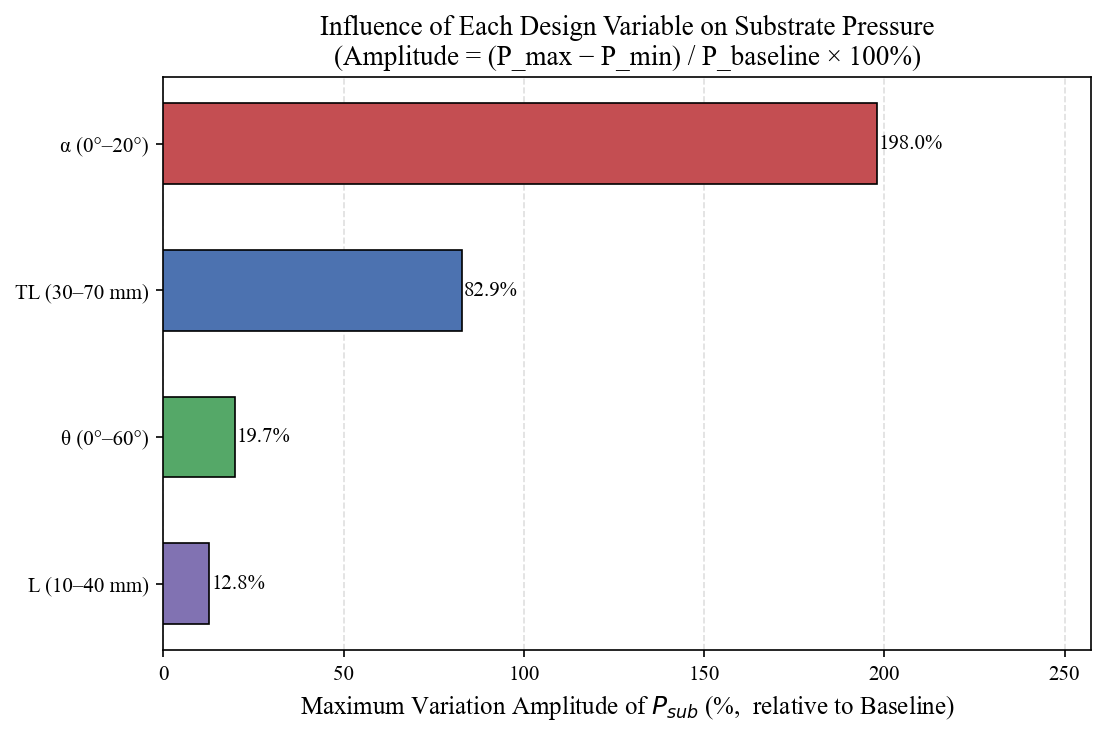
\includegraphics[width=0.75\textwidth]{figures/4.18.png}
  \caption{各参数对基底接触压力影响幅度对比柱状图}
  \label{fig:4.18}
\end{figure}

\cref{fig:4.18}以柱状图形式直观呈现了这一排序。$\alpha$的影响幅度远超其他变量，是调控基底接触压力最敏感的手段，但同时受到层高约束的强烈制约；$TL$以中等敏感性和充足的层高余量成为最具工程实用性的调控参数；$\theta$的影响幅度虽相对有限，但其兼具降低壁面剪切应力特性，具有独特工程价值；$L$的影响幅度最小且统计不显著，在工程设计中可视为次要参数。这一影响幅度排序为多目标优化提供了关键的先验信息，有助于理解NSGA-II优化结果中各参数趋向边界值的内在逻辑。

\subsection{Pearson相关分析}

为从统计学角度定量验证上述定性分析结论，对全部20个工况的四个设计变量与五项评价指标进行Pearson线性相关分析，结果如\cref{fig:4.19}、\cref{fig:4.20}所示。

\begin{figure}[!htb]
  \centering
  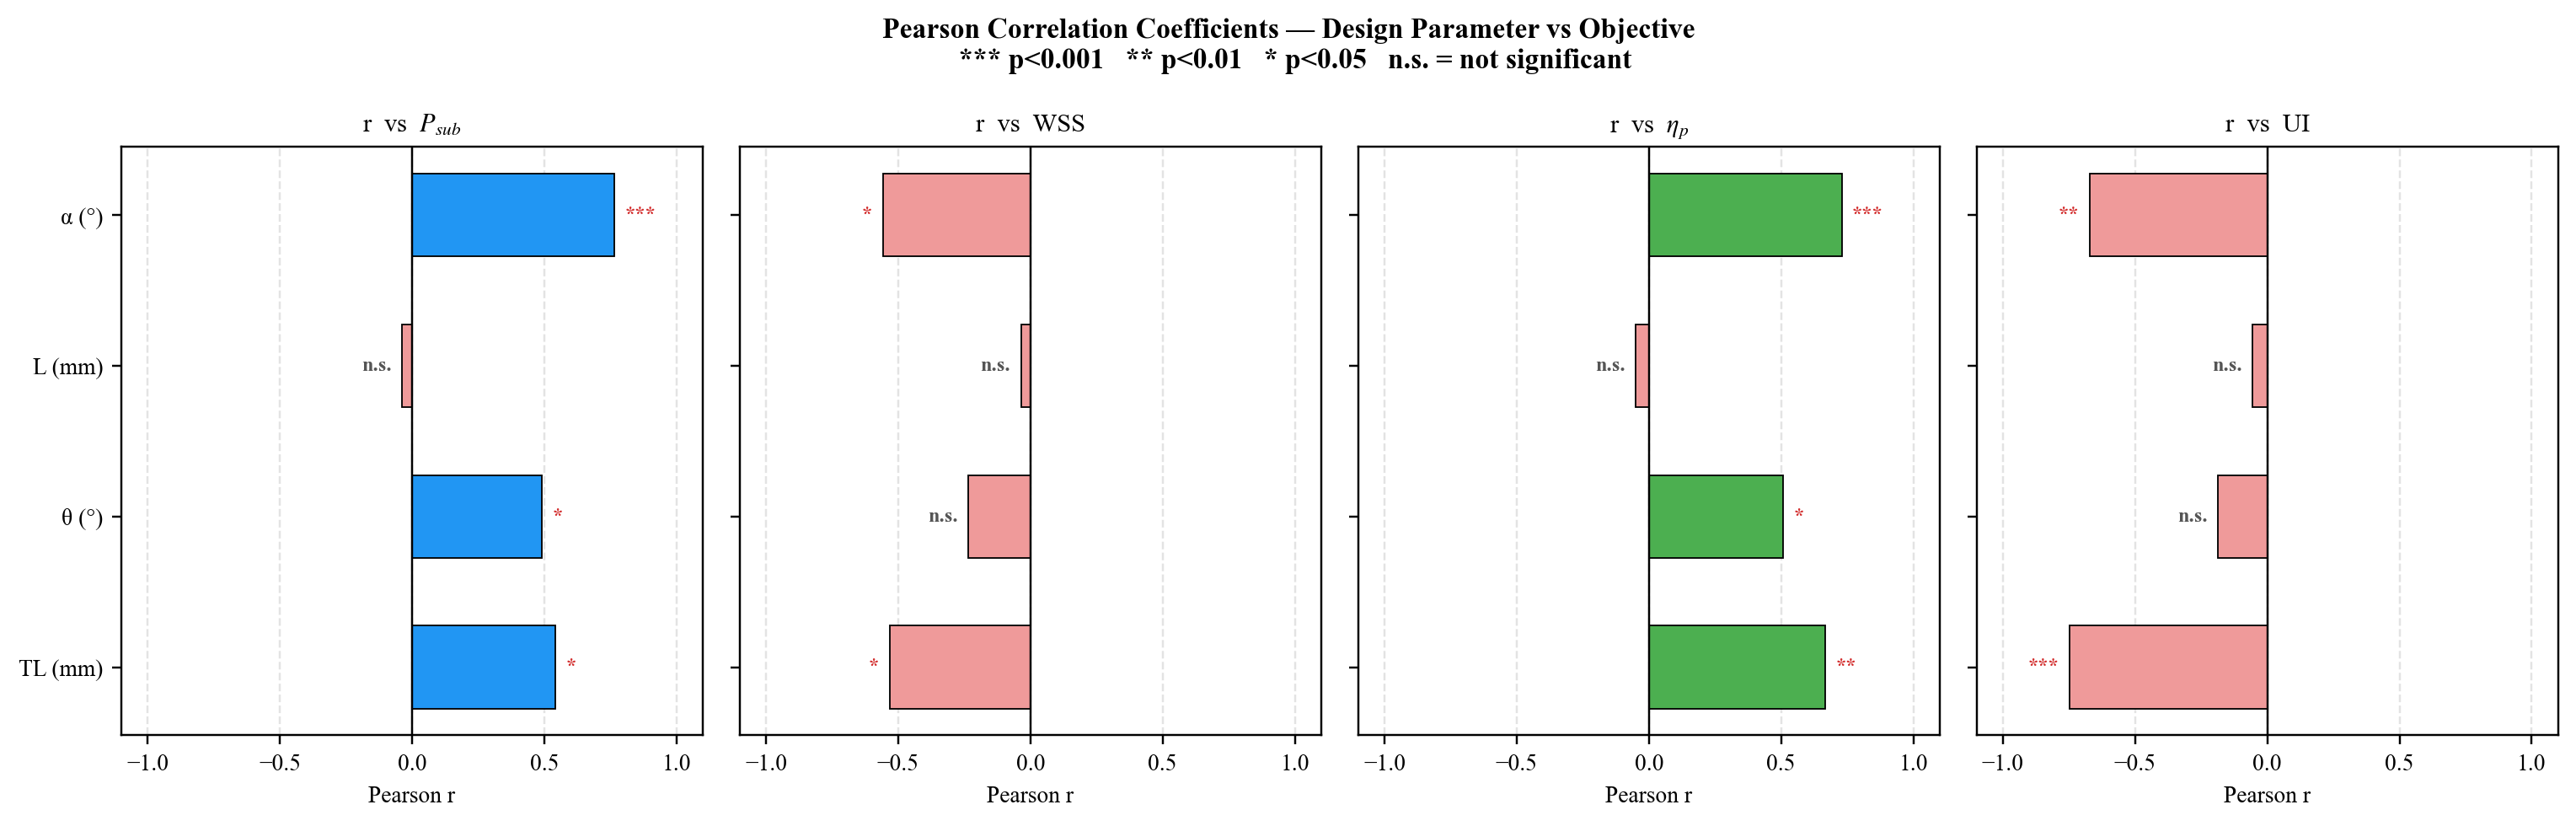
\includegraphics[width=0.8\textwidth]{figures/4.19.png}
  \caption{敏感性分析柱状图（前四项评价指标）}
  \label{fig:4.19}
\end{figure}

\begin{figure}[!htb]
  \centering
  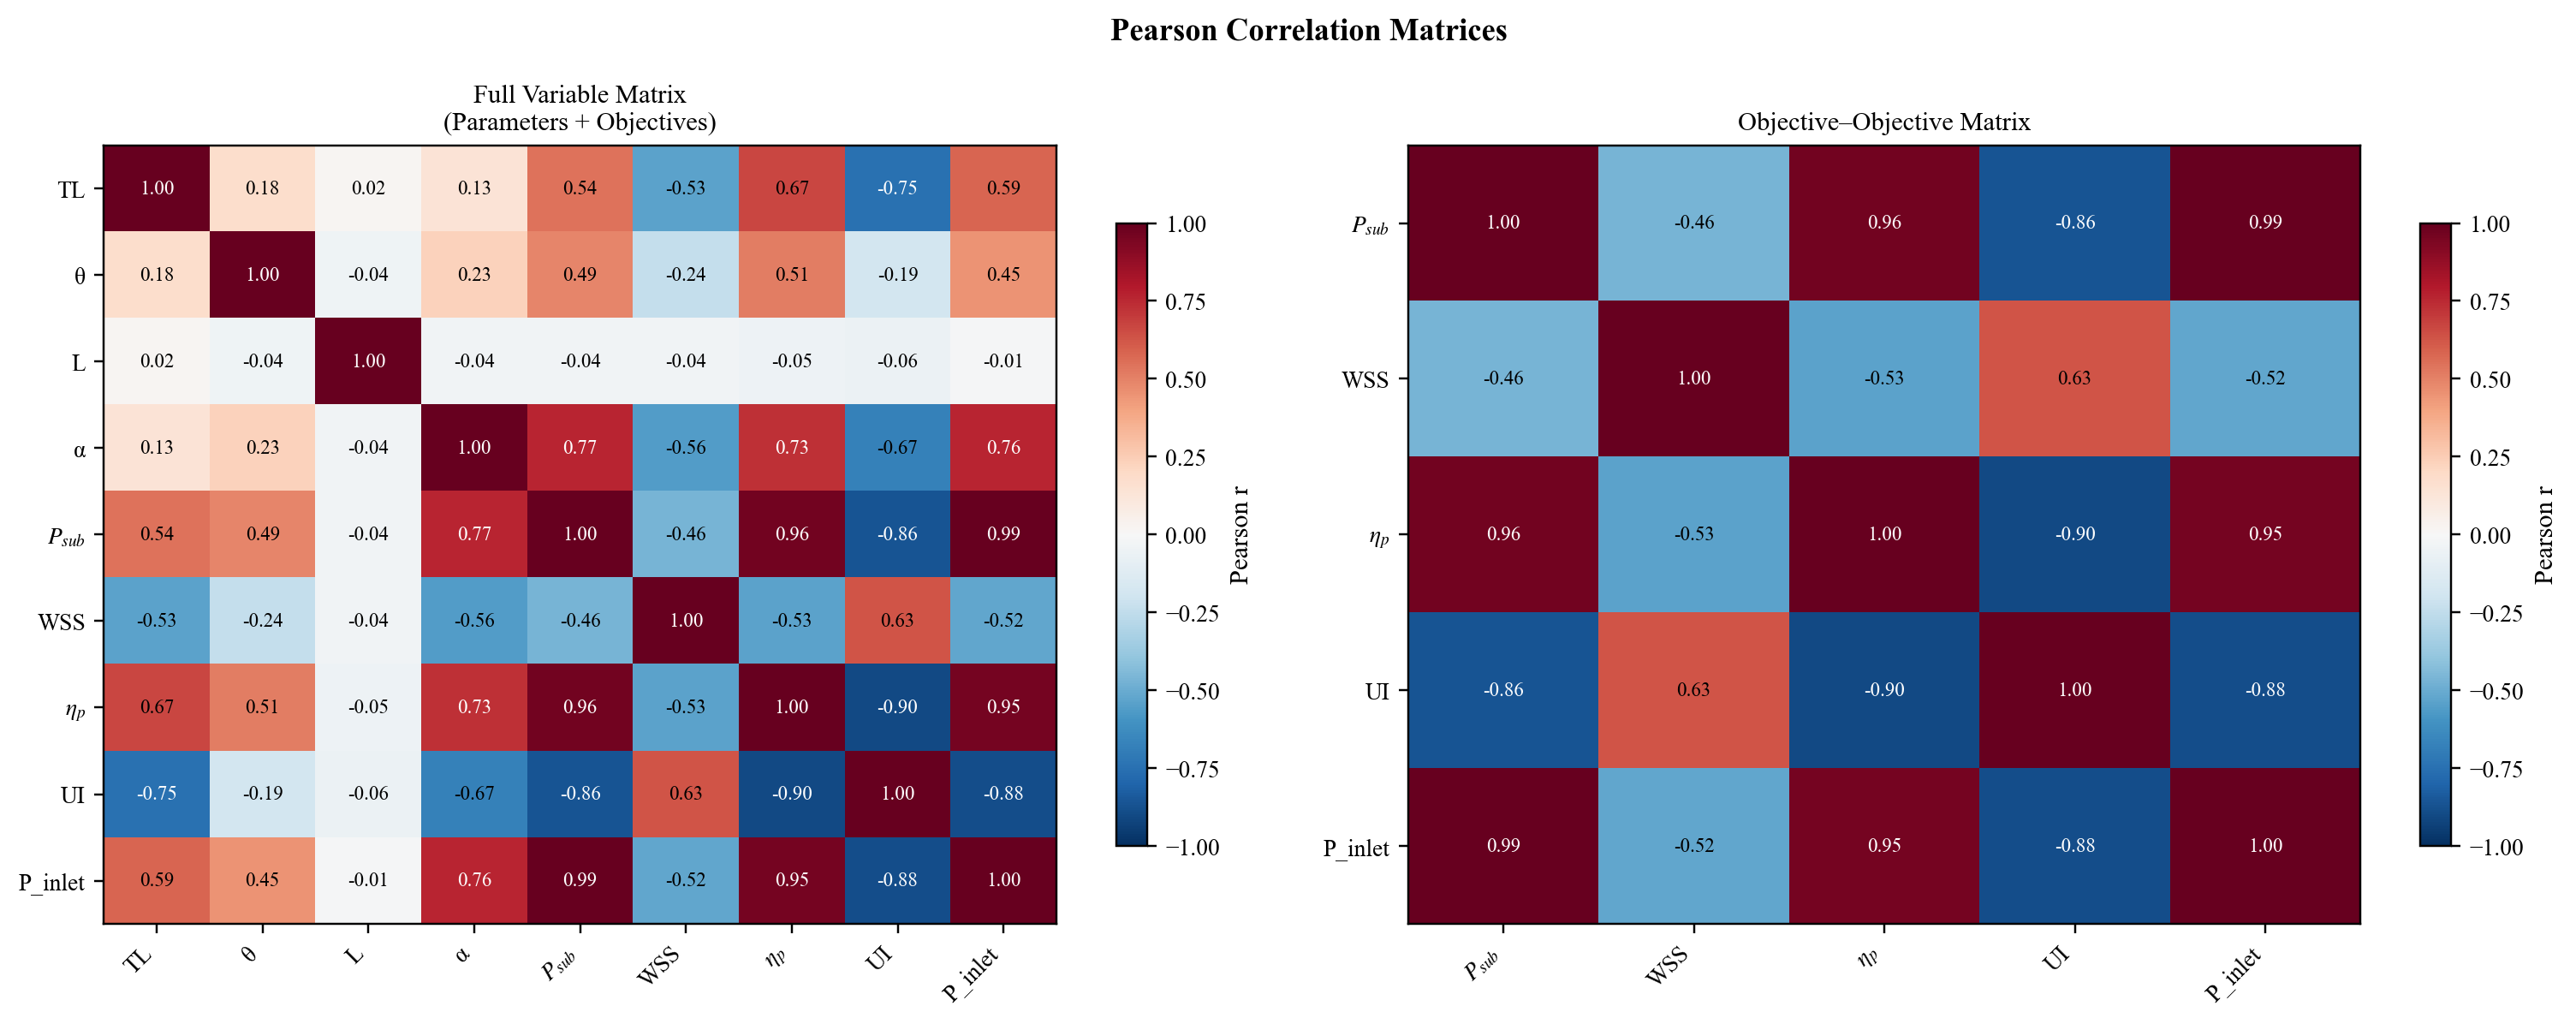
\includegraphics[width=0.95\textwidth]{figures/4.20.png}
  \caption{参数-目标全变量相关性热力图（左）、目标-目标相关性热力图（右）}
  \label{fig:4.20}
\end{figure}

对于核心指标$P_{sub,AWA}$，各变量的相关系数及显著性如\cref{tab:4.10}所示。这一结果与单因素极差分析的排序高度吻合，在统计层面上进一步证实了$\alpha$和$TL$是影响基底接触压力的显著参数，而$L$的影响在统计意义上可视为零，不宜作为主动调控手段。

\begin{table}[!htb]
  \centering
  \caption{$P_{sub,AWA}$相关系数与显著性汇总表}\label{tab:4.10}
  \renewcommand{\arraystretch}{1.3}
  \begin{tabular}{lcccc}
    \toprule
    \textbf{指标} & \textbf{Pearson r} & \textbf{Spearman r} & \textbf{P-value} & \textbf{Significance} \\
    \midrule
    $TL$       & $+0.541$ & $+0.746$ & 0.0137 & * \\
    $\theta$   & $+0.490$ & $+0.420$ & 0.0285 & * \\
    $L$        & $-0.038$ & $+0.080$ & 0.8726 & n.s. \\
    $\alpha$   & $+0.765$ & $+0.794$ & 0.0001 & *** \\
    \bottomrule
  \end{tabular}
\end{table}

目标-目标相关性热力图揭示了另一个具有工程意义的发现：$P_{inlet}$与$P_{sub,AWA}$之间的Pearson相关系数高达$r = 0.994$（$p < 0.001$），两者之间存在近乎完美的线性共线关系。这意味着在本研究的喷嘴-整形板系统中，提升基底接触压力与增大泵送入口压力是几乎等价的操作，两者无法独立解耦。
